%\documentclass[a4paper,12pt]{article}

\documentclass[
%  master,
  master=true,
  font=sans,
  printversion=false,
  joinlists=true,
  figures=true,
  tables=true,
  sourcecodes=false,
  theorems=false,
  bibencoding=utf8,
  language=czech,
  encoding=utf8,
  field=ainfk,
%  printversion,
  biblatex,
%  language=english,
%  font=sans,
  glossaries,
  index
]{kidiplom}

\usepackage[utf8]{inputenc}
\usepackage[czech]{babel}
\usepackage{listings}
\usepackage{graphicx}
\usepackage{verbatim}
\usepackage{titlesec}
\usepackage{fancyvrb}
\usepackage{hyperref}

\newcommand{\sectionbreak}{\clearpage}

\title{Implementace a testování linuxového plánovače úloh}
\title[english]{Task scheduler implementation and testing}

\begin{document}

\author{Kamil Kolakowski}
\supervisor{Mgr. Jan Outrata, Ph.D.}

\annotation{Tento text vzniknul jako studijní materiál pro techniky testující plánovač úloh ve firmě RedHat. Tento dokument obsahuje seznámení s plánovačem úloh jako komponentou jádra operačního systému, rozdělení úloh, seznámí nás s historií vývoje plánovačů na operačním systému Linux. Hlavní část tohoto dokumentu je tvořena popisem implementace současného plánovače úloh z jádra 3.18. Závěr tohoto textu je věnován popisu toho co na plánovači úloh testujeme a v úplném závěru jsou popsány výsledky jakých dosahujeme.}

\annotation[english]{This text was create as studing material for engineers of Redhat company who are testing task scheduler. This document includes introduction into task scheduler as component of operation system kernel, division tasks, explain us history of development of task scheduler on operation system Linux. Main part of this document includes implementation of present task scheduler from kernel version 3.18. Conclusion of this document is dedicated to explain what we are testing on task scheduler and in very end of this document is description what test results we achieve.}

\keywords{plánovač úloh; jádro; CFS; testování; vyvažování}
\keywords[english]{task scheduler; kernel; CFS; testing; balance}

\thanks{Děkuji vedoucímu práce Mgr. Janu Outratovi, Ph.D. za možnost vypracovat bakalářskou práci na toto téma, za jeho konzultace a různá doporučení. Dále bych rád poděkoval Ing. Radimu Krčmářovi za konzultace ohledně implementace plánovače a algoritmů vyvažování, Mgr. Jiřímu Horníčkovi za kontrolu gramatiky, Riku Van Rielovi za konzultování NUMA vyvažování a Volkeru Seekerovi, Dr. za poskytnutí materiálů věnovaných plánování na OS/Linux.}


%\tableofcontents
%\listoffigures

\maketitle

\section{Úvod}
Linuxový plánovač je jednou z nejdůležitějších komponent jádra každého operačního systému. Stará se o distribuci běžících úloh na systému, tak aby byly co nejlépe využity zdroje počítače. 

Paralelně s vývojem plánovače úloh dochází k vývoji technického vybavení počítačů. Práce na návhru současného plánovače úloh začala dříve, než se začaly prosazovat složitější architektury počítačů například s NUMA topologií. V tomto textu se proto podíváme, zda byl koncept plánovače doplněn o vyvažovaní úloh na strojích s podporou NUMA topologie. Na závěr dokumentu se podíváme na příklady, které demonstrují testování plánovače úloh. Testování provádíme za účelem nalezení možných problémů s plánováním a identifikaci slabin plánovače. 

Výstupy mého testování plánovače úloh používají ve firmě RedHat vývojáři plánovače úloh zejména pak Ing. Radim Krčmář a Rik van Riel. Testy, které používají vývojáři plánovače úloh, netestují komplexně všechny požadované vlastnosti plánovače. V současné době neexistuje jediný komplexní testovací nástroj, který by prověřil všechny požadované vlastnosti plánovače a to zejména férovost přidělování zdrojů, odezvu systému, celkovou propustnost a rovnoměrné vyvažování celého systému úlohami. K testování používáme modifikované verze testů Linpack, Stream, SPECjbb a PerfBench.

V textu popisuji plánovač, který je implementován do jader od verze 3.18.0. Poslední stabilní jádro s popisovanou implementací lze stáhout z adresy \linebreak https://www.kernel.org/pub/linux/kernel/v3.x/linux-3.18.1.tar.xz. 

Kód plánovače je v adresáři \verb#./linux-3.18.1/kernel/sched/#. Hlavním souborem implementující kostru plánovače je soubor \verb#core.c#. Dalšími důležitými soubory jsou \verb#fair.c# (implementující fair pravidla pro obyčejné úlohy), poté \verb#rt.c# (pravidla pro realtime úlohy), \verb#deadline.c# (pravidla pro úlohy konečného času). Další soubory jsou rozmístěny v mnoha dalších adresářích. Jedná se zejména o různé struktury, které jsou užívány i jinými komponentami jádra. Když ve svém popisu implementace plánovače narazím na funkci, nebo strukturu, doplním informaci o souboru, který ji obsahuje. Můj popis implementace by měl pomoct zorientovat se v kódu plánovače zájemci o hlubší studium tohoto algoritmu. Samotný popis funkcí ve zdrojovém kódu plánovače je velice technický a strohý.  

\section{Linuxové jádro, úloha plánovače, druhy úloh}

\subsection{Linuxové jádro a plánovač úloh}

Současné linuxové jádro je více úlohové. Jelikož je úloh na víceúlohových systémech často více než množství procesorů v systému, musí se úlohy o čas na procesoru dělit.
Plánovač úloh je algoritmus jádra systému, který se stará o co nejefektivněji využítí procesorového času.

Ačkoli byl Linux původně vyvíjen jako desktopový operační systém, dnes jej můžeme najít na serverech, vestavěných zařízeních, mainframech a superpočítačích. Zatížení úlohami se na jednotlivých platformách velice liší. Z tohoto důvodu a z důvodu prosazování se nových technologií jako je například multiprocessing, symetrický multithreading, nerovnoměrný přístup do paměti (NUMA), dochází k přehodnocování strategie přidělování zdrojů procesům. 

Každý plánovač také řeší rovnováhu mezi uživatelskou odezvou a obecnou férovostí. Po zamyšlení se nad výše jmenovanými vlastnosti a technologiemi je snadnější pochopit, jak složitý může být problém plánování úloh. 
\subsection{Procesy a vlákna}
Procesy jsou v Linuxu v rámci plánování brány jako skupiny vláken, které sdílí skupinu vláken (TGID). Jádro systému plánuje vždy zvlášť jednotlivé vlákno a ne proces. V celém mém dokumentu budu používat pojem úloha namísto vlákna nebo procesu.

\subsection{Členění úloh}
Úlohy si rozdělíme dle zdrojů, které požadují a podle toho jakým způsobem musí být plánovány, jelikož se v celém 
následujícím textu budeme věnovat jen jednomu typu úloh.

\subsubsection{Normální a úlohy reálného času}

Systém plánující úlohy reálného času (real time system) je takový systém, který garantuje doby odezvy systému na události, což znamená, že každá oparace by měla být dokončena v daném časovém období. Systém je klasifikován jako hard real time, pokud zmeškání lhůty může způsobit selhání systému a systém nazýváme soft real time v případě, že systém může tolerovat několik zmeškaných časových omezení. V běžném linuxovém jádru je podpora pouze pro soft real time úlohy (systém je soft real time). Real time úlohy mají v linuxovém plánovači svoji vlastní třídu pravidel (\verb#kernel/sched/rt.c#).

Ačkoli současný linuxový plánovač obsahuje i pravidla pro plánování úloh reálného času, nebudu se jim v této práci věnovat. Mnohem důležitější a v běžné praxi více používané jsou úlohy normální v rámci terminologie linuxového plánovače \verb#others tasks#.

Normální úlohy, které známe z desktopů, žádné časové omezení nemají.

\subsubsection{Úlohy CPU a I/O závislé}

Z hlediska plánování procesů rozdělujeme úlohy na úlohy závislé na vstupně výstupních zařízeních (zkráceně IO závislé) a na úlohy závislé na CPU. Některé úlohy tráví většinu času na CPU, na kterém dělají výpočty, jiné úlohy tráví hodně času tím, že čekají než se dokončí vstupní či výstupní operace, které jsou obvykle velmi pomalé. Operace I/O mohou čekat na vstup z klávesnice, disku nebo sítě. 
Záleží na tom na co je systém určen. Na desktopových systémech se často setkáváme s úlohami, které jsou I/O závislé. Na výpočetních serverech se pak setkáváme s úlohami, které jsou CPU závislé. 

Jelikož je Linux navržen tak, aby běžel na různých systémech, musí se umět vypořádat se všemi těmito úlohami. Úlohy, které běží dlouhou dobu, dokončí více práce na úkor odezvy systému. Jestliže naopak úloha běží krátkou dobu, systém může odpovědět rychleji na I/O požadavek, propustnost systému je nižší, protože v systému rostou režie plánovače na výměnu úloh. Plánovač musí proto hledat rovnováhu mezi odezvou a celkovou propustností systému. 

V této práci se zaměříme pouze na úlohy závislé na CPU.

\section{Předchůdci CFS}

\subsection{Vysvětlení pojmů}

\noindent
 

\begin{itemize}

\item První plánovač (jádro verze 1.2, rok 1995) byl založený na round robin plánovací technice. \textbf{Round Robin} plánovací technika je založena na tom, že je úloze dané časové kvantum po které může běžet na procesoru. Až toto kvantum uplyne je úloze odebrán procesor a je spuštěna další úloha. Takto dokola se postupně střídají všechny úlohy ve frontě běžících úloh. To znamená, že pořadí se nemění a úlohy jsou postupně jadna po druhé dokola spouštěny. Z tohoto minimalistického návrhu plynula jednoduchost a rychlost, ale nebylo to komplexní řešení plánování, nebyl zaměřen na architektury s mnoha procesory ani na architektury s podporou více vláken.

\item U plánovače úloh od verze jádra 2.2 (rok 1999) došlo k implementaci tříd plánování, umožňující používat rozdílná pravidla pro real-time úlohy, non-preemtable úlohy (úlohy které běžely dokud samy neskončily) a non-realtime úlohy (obyčejné úlohy, s preempcí).

\item Jádro 2.4 (rok 2001) má jednoduchý plánovač O(N) operující s lineární časovou složitostí (rostoucími počty úloh rostla stejně i doba práce plánovače). Plánovač rozdělil čas do epoch a v rámci této epochy bylo úloze povoleno běžet její časové kvantum. Jestliže úloha nepoužila celé své časové kvantum, pak polovina zbývajícího času byla přičtena k novému časovému kvantu, aby mohla úloha běžet déle v další časové epoše. Plánovač přes všechny úlohy aplikoval funkci goodness k zjištění jakou úlohu má spustit jako další. Ačkoli toho lze dosáhnout snadno, byl příliš neefektivní, postrádal škálovatelnost a byl špatný na úlohy reálného času. Jeho další slabinou bylo postrádání podpory pro nové hardwarové architektury jako jsou třeba více jádrové procesory. 

\item Prvním plánovačem na jádrech verze 2.6 (rok 2003) byl plánovač zvaný O(1), který byl navržen k řešení mnoha problémů 2.4 plánovače. \linebreak Nejdůležitější změnou bylo, že plánovač již nezahrnoval identifikaci další úlohy pro spuštění (a nutnost opakovaně procházet všechny úlohy, aby zjistil, kterou má spustit nejdřív), z čehož plynulo i jeho jméno O(1), což znamená, že pracoval v konstantní časovou složitostí a byl více škálovatelný. O(1) plánovač uchovával záznamy o běžících úlohách ve frontách běžících úloh (front bylo více pro každou úroveň priorit dvě – jedna pro aktivní úlohy, druhá pro expirované úlohy), které používal pro výběr, jakou úlohu bude provádět jako další. Plánovač také zahrnoval měření interaktivity s množstvím heuristiky, která způsobila, že byl plánovač těžkopádný. Plánovač zvýhodňoval interaktivní úlohy před dávkovými (batch) úlohami.

\end{itemize}

\section{Completely fair scheduler}% - úplně férový plánovač}

Byl poprvé použit v jádrech 2.6.23 v roce 2008. Autorem je Ingo Molnár autor O(1) plánovače. Asymptotická časová složitost plánovacího algoritmu je O(log N), přičemž samotné naplánování sice probíhá v konstantním čase, ale znovuzařazení procesu do červeno-černého stromu vyžaduje O(log N) operací. Od svých předchůdců se liší zejména tím, že jsou zcela oddělena plánovací pravidla od kostry plánovače. Tímto vznikl prostor, zejména pro lidi z komunity, vytvořit si vlastní plánovací pravidla. O něco později byly do plánovače implementovány algoritmy na NUMA vyvažování. Spolu s nimi byla do algoritmu plánovače zavlčena heuristika, za pomocí které například odhadujeme na jaké NUMA uzly úloha přistupuje. V současné době jsou v CFS podporovány architektury s multiprocesingem, symetrickým multithreadingem, počítače s podporou NUMA technologie a virtualizace. Plánovač CFS je použit na všech architekturách dostupných na OS Linux. Samotná plánovací technika je založená na velice jednoduchém principu. Ve stromu běžících úloh jsou seřazeny úlohy podle toho kolik času jim bylo dosud přiděleno k běhu. Úloha, které má toto množství menší než současně běžící úloha je naplánována jako další. Pro každý procesor udržuje plánovač jednu frontu běžících úloh (červeno-černý strom). Další podrobnosti o fungování algoritmu si vysvětlíme v další části tohoto textu.

\subsection{Kostra plánovače}
Vstupní branou do linuxového plánovače úloh je funkce \verb#schedule()#, která je definovaná v \verb#kernel/sched/core.c# (v dřívějších jádrech v \verb#/kernel/sched.c#). Tuto funkci používá jádro k vyvolání procesu plánovače, který rozhoduje o tom, která úloha se má spustit a poté realizuje její spuštění. 

%\begin{lstlisting}[language=c]
%
%static void __sched __schedule(void)
%{
%        struct task_struct *prev, *next;
%        unsigned long *switch_count;
%        struct rq *rq;
%        int cpu;
%
%need_resched:
%        preempt_disable();
%        cpu = smp_processor_id();
%        rq = cpu_rq(cpu);
%        rcu_note_context_switch(cpu);
%        prev = rq->curr;
%
%        schedule_debug(prev);
%
%        if (sched_feat(HRTICK))
%                hrtick_clear(rq);
%
%        /*
%         * Make sure that signal_pending_state()->signal_pending() below
%         * can't be reordered with __set_current_state(TASK_INTERRUPTIBLE)
%         * done by the caller to avoid the race with signal_wake_up().
%         */
%        smp_mb__before_spinlock();
%        raw_spin_lock_irq(&rq->lock);
%
%        switch_count = &prev->nivcsw;
%        if (prev->state && !(preempt_count() & PREEMPT_ACTIVE)) {
%                if (unlikely(signal_pending_state(prev->state, prev))) {
%                        prev->state = TASK_RUNNING;
%                } else {
%                        deactivate_task(rq, prev, DEQUEUE_SLEEP);
%                        prev->on_rq = 0;
%
%                        /*
%                         * If a worker went to sleep, notify and ask workqueue
%                         * whether it wants to wake up a task to maintain
%                         * concurrency.
%                         */
%                        if (prev->flags & PF_WQ_WORKER) {
%                                struct task_struct *to_wakeup;
%
%                                to_wakeup = wq_worker_sleeping(prev, cpu);
%                                if (to_wakeup)
%                                        try_to_wake_up_local(to_wakeup);
%                        }
%                }
%                switch_count = &prev->nvcsw;
%        }
%
%        if (task_on_rq_queued(prev) || rq->skip_clock_update < 0)
%                update_rq_clock(rq);
%
%        next = pick_next_task(rq, prev);
%        clear_tsk_need_resched(prev);
%        clear_preempt_need_resched();
%        rq->skip_clock_update = 0;
%
%        if (likely(prev != next)) {
%                rq->nr_switches++;
%                rq->curr = next;
%                ++*switch_count;
%
%                context_switch(rq, prev, next); /* unlocks the rq */
%                /*
%                 * The context switch have flipped the stack from under us
%                 * and restored the local variables which were saved when
%                 * this task called schedule() in the past. prev == current
%                 * is still correct, but it can be moved to another cpu/rq.
%                 */
%                cpu = smp_processor_id();
%                rq = cpu_rq(cpu);
%        } else
%                raw_spin_unlock_irq(&rq->lock);
%
%        post_schedule(rq);
%
%        sched_preempt_enable_no_resched();
%        if (need_resched())
%                goto need_resched;
%}
%
%
%\end{lstlisting}

Jelikož je linuxové jádro pre-emptivní, může se stát, že je úloha přerušena v režimu jádra úlohou s vyšší prioritou. Zastavená úloha v nedokončené operaci v režimu jádra může pokračovat, až když je znova naplánována. 

Proto první věc kterou funkce \verb#schedule()# udělá je, že vypne pre-emptci, takže úloze nemůže být odebráno CPU během kritických operací. 
\begin{verbatim}
preempt_disable();
\end{verbatim}
Dále je pak uzamčena fronta úloh na aktuálním CPU, jelikož pouze jedné úloze je povoleno modifikovat frontu úloh.
\begin{verbatim}
raw_spin_lock_irq(&rq->lock);
\end{verbatim}
Potom funkce schedule() zjišťuje stav úlohy, která běžela jako předchozí. Jestliže současná úloha již nechce běžet a zároveň je povolena preemptce, pak může být úloha odebrána z běžící fronty. 
\begin{verbatim}
if (prev->state && !(preempt_count() & PREEMPT_ACTIVE)) {
\end{verbatim}
Jestliže úloha přijala neblokovaný signál, pak je její stav nastaven na běžící a úloha je ponechána ve frontě běžících úloh. Takže současná úloha má šanci být naplánována znova. 
\begin{verbatim}
if (unlikely(signal_pending_state(prev->state, prev))) {
   prev->state = TASK_RUNNING;
\end{verbatim}
K odebrání úlohy z fronty úloh voláme funkci \verb#deactivate_task#, která interně volá \verb#dequeue_task()# pro danou plánovací třídu.
\begin{verbatim}
deactivate_task(rq, prev, DEQUEUE_SLEEP);
\end{verbatim}
Dále voláme \verb#pick_next_task# k výběru další vhodné úlohy, která bude spuštěna na CPU. 
\begin{verbatim}
next = pick_next_task(rq, prev);
\end{verbatim}
Poté dojde k vyčištění dvou příznaků (proměnných) sloužících k vyvolání funkce \verb#schedule()#. Tyto příznaky jsou součástí \verb#task_struct# a jsou pravidelně jádrem kontrolovány. 
\begin{verbatim}
clear_tsk_need_resched(prev);
clear_preempt_need_resched();
\end{verbatim}
%\begin{lstlisting}
%
%pick_next_task(struct rq *rq, struct task_struct *prev)
%{       
%	const struct sched_class *class = &fair_sched_class;
%        	struct task_struct *p;
%        /*
%         * Optimization: we know that if all tasks are in
%         * the fair class we can call that function directly:
%         */
%        if (likely(prev->sched_class == class &&
%                   rq->nr_running == rq->cfs.h_nr_running)) {
%                p = fair_sched_class.pick_next_task(rq, prev);
%                if (unlikely(p == RETRY_TASK))
%                        goto again;
%                
%                /* assumes fair_sched_class->next == idle_sched_class */
%                if (unlikely(!p))
%                        p = idle_sched_class.pick_next_task(rq, prev);
%                
%                return p;
%        }
%
%again:  
%        for_each_class(class) {
%                p = class->pick_next_task(rq, prev);
%                if (p) {
%                        if (unlikely(p == RETRY_TASK))
%                                goto again;
%                        return p;
%                }
%        }
%        
%        BUG(); /* the idle class will always have a runnable task */
%}
%
%\end{lstlisting}

Funkce \verb#pick_next_task# je také implementována v \verb#kernel/sched/core.c#. Prochází plánovací třídy a hledá třídu s největší prioritou, která má spustitelnou úlohu.
% for_each_class
\begin{verbatim}
for_each_class(class) {
   p = class->pick_next_task(rq, prev);
\end{verbatim}
Jelikož je většina úloh obsluhována pomocí třídy \verb#fair_sched_class#, je zkratka do této třídy implementována na hned začátku funkce \verb#pick_next_task()#.
\begin{verbatim}
if (likely(prev->sched_class == class &&
   rq->nr_running == rq->cfs.h_nr_running)) {
\end{verbatim}
Takže schedule() zkontroluje jestli \verb#pick_next_task()# našla novou úlohu nebo vzala úlohu, která již běžela předtím.
\begin{verbatim}
if (likely(prev != next)) {
\end{verbatim}
Jestliže našla úlohu, která běžela předtím nechá ji běžet dál. Jestliže plánovač vybere úlohu, která předtím neběžela, je volána volána funkce s samovysvětlujícím názvem \verb#context_switch#. V rámci context switche dochází k výměně stavu registrů, zásobníku a je přemapována paměť.
\begin{verbatim}
context_switch(rq, prev, next); /* unlocks the rq */
\end{verbatim}

\begin{figure}[p]
\center
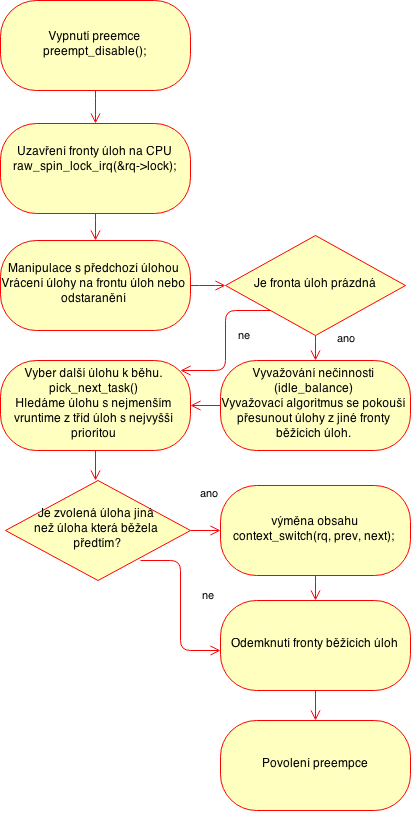
\includegraphics[scale=0.7]{obrazky/kostraPlanovace.png}
\caption{Diagram algoritmu kostry plánovače}
\label{kostra planovace}
\end{figure}

\newpage
\subsection{Plánovací třídy}
Každá úloha patří do určité třídy plánování, která určuje, jakým způsobem bude úloha naplánována. 
Současný plánovač byl navržen tak, aby bylo možno používat rozšířenou hierarchii modulů. Jednotlivé moduly jsou zapouzdřením plánovacích pravidel, které používá kostra plánovače. 
Plánovací třída definuje sadu funkcí prostřednictvím \verb#sched_class# (v \verb#kernel/sched/sched.h#), které definují chování plánovače.\newline 

\noindent
Každá třída plánování poskytuje funkce jako:
\begin{itemize}
\item \verb#enqueue_task# (...) 
Je volána, když se úloha stává spustitelnou. Vkládá plánovací entitu (úlohu) do fronty běžících úloh (ve fair třídě do červeno-černého stromu) a zvýší hodnotu proměnnou \verb#nr_running# o 1.
\item \verb#dequeue_task# (...) 
Pokud úloha není dále spustitelná, je volána tato funkce, aby vyjmula danou plánovací entitu (úlohu) z fronty běžících úloh (v fair plánovací třídě z červeno-černého stromu). Sníží se hodnota proměnné \verb#nr_running# o 1.
\item \verb#yield_task# (...) 
Tato funkce je v podstatě stejná jako předchozí. Vyjme úlohu a následně ji zařadí, není-li \verb#compat_yield# sysctle (utilita užívaná ke změně parametrů jádra za běhu systému) zapnutý. V tomto případě umístí plánovací entitu (úlohu) do fronty běžících úloh (ve fair třídě nejvíce napravo do červeno-černém stromu).
\item \verb#check_preempt_curr# (...) 
Tato funkce kontroluje, zda úkol, který se dostal do spustitelného stavu, může odebrat současně běžící úlohu.
\item \verb#pick_next_task# (...) 
Tato funkce vybírá nejvhodnější úlohu způsobilou ke spuštění jako další.
\item \verb#set_curr_task# (...) 
Tato funkce je volána, jestliže se změní plánovací třída úlohy, nebo změní-li se skupina úlohy.
\item \verb#task_tick# (...) 
Tato funkce je většinou volána z \verb#time_tick()# funkce a může vést k výměně úloh. Řídí běh preempce. \newline
\end{itemize}

Všechny existující plánovací třídy jsou v linuxovém jádru seřazeny v seznamu podle priorit plánovacích tříd. První proměnná ve struktuře \verb#sched_task# se nazývá \verb#next# a je ukazatelem na plánovací třídu s nižší prioritou. Seznam je užíván k preferenci úloh jednoho typu před druhým. V současnosti vypadá seznam tříd následovně
%$$ 
%stop\_sched\_class \rightarrow dl\_sched\_class \rightarrow rt\_sched\_class \rightarrow fair\_sched\_class \rightarrow idle\_sched\_class \rightarrow NULL 
%$$

$$ 
stop\_class \rightarrow dl\_class \rightarrow rt\_class \rightarrow fair\_class \rightarrow idle\_class \rightarrow NULL 
$$

\verb#Stop# a \verb#idle# jsou speciální třídy plánování. \verb#Stop# slouží k naplánování úlohy, která zastaví úlohu běžící na CPU a která a nemůže být přerušena žádnou jinou úlohou. Přerušená může být pouze obsluhou přerušení. Příkladem úloh plánovanými dle třídy stop jsou úlohy které vyvažují fronty běžících úloh. \verb#idle# slouží k naplánování nečinné úlohy na CPU, která je naplánovaná pouze v případě, že neexistuje jiná úloha k běhu. Třída \verb#dl(deadline)# je pro plánování úloh s určeným termínem ukončení, třída \verb#rt(real-time)# je pro plánování úloh reálného času a \verb#fair# slouží pro plánování běžných úloh.

Úloze lze specifikovat třídu plánování pomocí systémové utility \verb#chrt# nebo pomocí API, které je popsáno podrobně na manuálových stránkách \verb#man sched#.

%\subsection{Funkce schedule() je volána}
\subsection{Volání plánovače}

K volání plánovače úloh dochází prostřednictvím funkce schedule() z těchto tří důvodů:

\subsubsection{Pravidelné volání k aktualizaci vruntime u právě běžící úlohy}

Přerušení od časovače pravidelně volá fuknci \verb#scheduler_tick()# \linebreak (z \verb#kernel/sched/core.c#). Dochází k aktualizaci hodnoty vruntime a také ke změnám na aktuální frontě úloh (vše 1000 krát za sekundu). V kódu funkce \newline \verb#scheduler_tick()# je aktualizace realizována voláním 
\begin{verbatim}
curr->sched_class->task_tick(rq, curr, 0);
\end{verbatim}
Takto volaná aktualizace nám zaručuje aktualizaci údajů dle pravidel dané třídy, ve které byla úloha spuštěna. Ve funkci \verb#scheduler_tick()# jsou volání 
\begin{verbatim}
rq->idle_balance = idle_cpu(cpu);
trigger_load_balance(rq);
\end{verbatim}
která zajištují vyvážení zátěže v případě, že máme je systém s více CPU.

%Funkce scheduler\_tick() (z kernel/sched/core.c) je volána pomocí časovače přerušení. 
%Aktualizuje u běžící úlohy vruntime a díky změně dojde k aktualizaci běžící fronty.
% curr->sched_class->task_tick

%\begin{lstlisting}
%
%scheduler_tick(void)
%{
%	int cpu = smp_processor_id();
%	struct rq *rq = cpu_rq(cpu);
%	struct task_struct *curr = rq->curr;
%
%	sched_clock_tick();
%
%	raw_spin_lock(&rq->lock);
%	update_rq_clock(rq);
%	curr->sched_class->task_tick(rq, curr, 0);
%	update_cpu_load_active(rq);
%	raw_spin_unlock(&rq->lock);
%
%	perf_event_task_tick();
%
%#ifdef CONFIG_SMP
%	rq->idle_balance = idle_cpu(cpu);
%	trigger_load_balance(rq);
%#endif
%	rq_last_tick_reset(rq);
%}
%
%\end{lstlisting}

%Volání 
%\begin{lstlisting} 
%rq -> idle_balance = idle_cpu(cpu) 
%\end{lstlisting} 
%a 
%\begin{lstlisting} 
%trigger_load_balance(rq) 
%\end{lstlisting} 
%nám pak zajišťují vyvážení zatížení pro případ, že máme nakonfigurován SMP.
%
\subsubsection{Když současně běžící úloha usne}

Úloha která je uspávána, čeká na specifickou událost, je implementována podobně jako následující ukázka, kterou lze najít v různých částech linuxového jádra.

%\begin{verbatim} 
%DEFINE_WAIT(wait); 
%
%add_wait_queue(q, &wait); 
%while (!condition) /* waiting for event */
%{ 
%     prepare_to_wait(&q, &wait, TASK_INTERRUPTIBLE); 
%     schedule(); 
%} 
%finish_wait(&q, &wait);
%\end{verbatim}
%\pagebreak 
Úloha vytvoří čekací frontu a přidá se do ní. 
\nopagebreak
\begin{verbatim}
DEFINE_WAIT(wait);
add_wait_queue(q, &wait);
\end{verbatim}
Ve smyčce pak čeká, než je splněna podmínka. Ve smyčce dojde k nastavení statusu úlohy na TASK\_INTERRUPTIBLE nebo TASK\_UNITERRUPTIBLE. Poté dojde k zavolání plánovače a úloha se uspí. Plánovač odstraní úlohu z běžící fronty. Úloha čeká na jinou úlohu, která zavolá funkci \verb#wake_up(&wait)#.
 
\begin{verbatim}
while (!condition) /* waiting for event */
{ 
     prepare_to_wait(&q, &wait, TASK_INTERRUPTIBLE); 
     schedule(); 
} 

finish_wait(&q, &wait);
\end{verbatim}

Nastane-li potřebná událost (podmínka condition), je ukončena smyčka a úloha je odstraněna z čekací fronty. 

\subsubsection{Při probuzení spící úlohy}

%Spící úloha obvykle očekává kód, který volá funkci wake\_up na patřičné čekací frontě, která finálně volá funkci try\_to\_wake\_up(). Samotné probuzení obstarává funkce ttwu\_queue, jejíž volání je na konci funkce try\_to\_wake\_up(). 

Spící úloha obvykle očekává kód, který volá funkci \verb#wake_up# na patřičné čekací frontě. Postupně je volána hierarchie funkcí, až dojde na volání \verb#ttwu_queue# z \verb#try_to_wake_up()#. Ta obstará samotné probuzení úlohy.  

%Funkce dělá následující tři věci:
%Kód postupně dělá následující:
Postupně dochází k následujícím činnostem
\begin{enumerate}
\item V případě, že úloha ještě není ve frontě běžících úloh, dojde k vrácení úlohy do této fronty. Toto je realizováno pomocí funkce \verb#tttwu_queue#, která zavře frontu běžících úloh a zavolá \verb#ttwu_do_activate()#.
\item Probudí úlohu pomocí nastavení stavu na TASK\_RUNNING (ve funkci \newline \verb#ttwu_do_wakeup()#).
\item Jestliže má probuzená úloha větší prioritu než úloha současně běžící, je nastaven \verb#need_resched# příznak pro vyvolání funkce \verb#schedule()#. Toto je také realizováno z funkce \verb#ttwu_do_wakeup()#.
\end{enumerate}

%\begin{lstlisting} 
%
%/*
% * Return: %true if @p was woken up, %false if it was already running.
% * or @state didn't match @p's state.
% */
%static int
%try_to_wake_up(struct task_struct *p, unsigned int state, int wake_flags)
%{
%        unsigned long flags;
%        int cpu, success = 0;
%
%        /*
%         * If we are going to wake up a thread waiting for CONDITION we
%         * need to ensure that CONDITION=1 done by the caller can not be
%         * reordered with p->state check below. This pairs with mb() in
%         * set_current_state() the waiting thread does.
%         */
%        smp_mb__before_spinlock();
%        raw_spin_lock_irqsave(&p->pi_lock, flags);
%        if (!(p->state & state))
%                goto out;
%
%        success = 1; /* we're going to change ->state */
%        cpu = task_cpu(p);
%
%        if (p->on_rq && ttwu_remote(p, wake_flags))
%                goto stat;
%
%#ifdef CONFIG_SMP
%        /*
%         * If the owning (remote) cpu is still in the middle of schedule() with
%         * this task as prev, wait until its done referencing the task.
%         */
%        while (p->on_cpu)
%                cpu_relax();
%        /*
%         * Pairs with the smp_wmb() in finish_lock_switch().
%         */
%        smp_rmb();
%
%        p->sched_contributes_to_load = !!task_contributes_to_load(p);
%        p->state = TASK_WAKING;
%
%        if (p->sched_class->task_waking)
%                p->sched_class->task_waking(p);
%
%        cpu = select_task_rq(p, p->wake_cpu, SD_BALANCE_WAKE, wake_flags);
%        if (task_cpu(p) != cpu) {
%                wake_flags |= WF_MIGRATED;
%                set_task_cpu(p, cpu);
%        }
%#endif /* CONFIG_SMP */
%
%        ttwu_queue(p, cpu);
%stat:
%        ttwu_stat(p, cpu, wake_flags);
%out:
%        raw_spin_unlock_irqrestore(&p->pi_lock, flags);
%
%        return success;
%}
%
%
%static void ttwu_queue(struct task_struct *p, int cpu)
%{
%        struct rq *rq = cpu_rq(cpu);
%
%#if defined(CONFIG_SMP)
%        if (sched_feat(TTWU_QUEUE) && !cpus_share_cache(smp_processor_id(), cpu)) {
%                sched_clock_cpu(cpu); /* sync clocks x-cpu */
%                ttwu_queue_remote(p, cpu);
%                return;
%        }
%#endif
%
%        raw_spin_lock(&rq->lock);
%        ttwu_do_activate(rq, p, 0);
%        raw_spin_unlock(&rq->lock);
%}
%
%
%static void
%ttwu_do_activate(struct rq *rq, struct task_struct *p, int wake_flags)
%{
%#ifdef CONFIG_SMP
%        if (p->sched_contributes_to_load)
%                rq->nr_uninterruptible--;
%#endif
%
%        ttwu_activate(rq, p, ENQUEUE_WAKEUP | ENQUEUE_WAKING);
%        ttwu_do_wakeup(rq, p, wake_flags);
%}
%
%static void
%ttwu_do_wakeup(struct rq *rq, struct task_struct *p, int wake_flags)
%{
%        check_preempt_curr(rq, p, wake_flags);
%        trace_sched_wakeup(p, true);
%
%        p->state = TASK_RUNNING;
%#ifdef CONFIG_SMP
%        if (p->sched_class->task_woken)
%                p->sched_class->task_woken(rq, p);
%
%        if (rq->idle_stamp) {
%                u64 delta = rq_clock(rq) - rq->idle_stamp;
%                u64 max = 2*rq->max_idle_balance_cost;
%
%                update_avg(&rq->avg_idle, delta);
%
%                if (rq->avg_idle > max)
%                        rq->avg_idle = max;
%
%                rq->idle_stamp = 0;
%        }
%#endif
%}
%
%
%\end{lstlisting} 

\newpage
\subsection{Fair plánovací třída}

Zcela férový plánovač, je nejčastěji používaný pro kategorii normálních (v terminologii CFS others) úloh. Užívá plánovací pravidla z třídy fair (kterou lze najít v \verb#kernel/sched/fair.c#).
CFS je postaven na myšlenkách ideálního mnoho úlohového procesoru. Ideální mnoho úlohový procesor je pak takový, na kterém běží paralelně všechny aktivní úlohy a každá úloha tak dostává adekvátní porci procesorového výkonu. Takže například pro 2 úlohy běžící na jednom ideálním mnoho úlohovém systému by každá úloha dostala 50\% výkonu procesoru. 


\begin{figure}[ht]
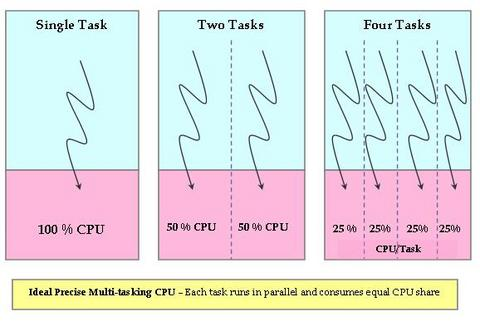
\includegraphics[scale=1.0]{obrazky/idealProcessor.jpg}
\caption{Schéma ideálního procesoru}
\label{idealni procesor}
\end{figure}


Mnoho úlohový ideální systém, je čistě abstraktní model a není z fyzikálního hlediska možný. Ale koncept CFS je založen na stejném cíli a to přidělení všem běžícím úlohám férové množství procesoru. Současný plánovač tudíž nenabízí každé úloze stejnou část výkonu procesoru, ale snaží se docílit, aby úlohy běžely na CPU stejné časové kvantum. 

\begin{figure}[ht]
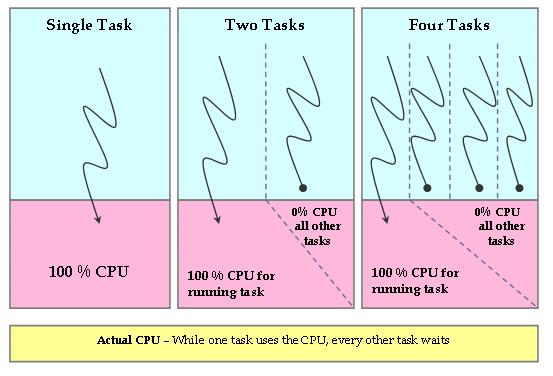
\includegraphics[scale=0.85]{obrazky/realProcessor.jpg}
\caption{Schéma reálného procesoru}
\label{realny procesor}
\end{figure}


V CFS byl klasický model předchozích plánovačů založených na obdobích (epochs) a pevně daných časových úsecích (time slices) zcela předělán. Byl zaveden virtual runtime počítadlo pro každou úlohu, které nám udává hodnotu času stráveného na procesoru vynásobenou koeficientem priority. CFS odkazuje na vruntime (\verb#p->se.vruntime# kde p je struktura \verb#sched_entity#).  
Když se zjistí, že některá úloha z fronty běžících úloh strávila na procesoru méně času než ta právě běžící, dojde k naplánování běhu úlohy s menší hodnotou vruntime. Místo aby plánovač udržoval úlohy ve frontě, jako to dělali předchůdci CFS plánovače, CFS udržuje časově seřazený červeno-černý strom. Je samovyvažovací a neexistuje v něm cesta, která je více než dvojnásobně delší než kterákoli jiná v daném stromu. Druhá vlastnost je, že přidání úlohy do stromu, odebrání úlohy ze stromu a výběr úlohy ze stromu probíhá v O(log n) čase (kde n je počet uzlů v daném stromu).

Úlohy (representovanými \verb#sched_entity# objekty) jsou na stromu seřazeny dle hodnot ve vruntime. Úlohy s nejvyšší potřebou běhu na CPU jsou uloženy na nejvíce levé části stromu a úlohy s nejnižší potřebou běhu na CPU jsou uloženy ve stromě nejvíc napravo.

\begin{figure}[ht]
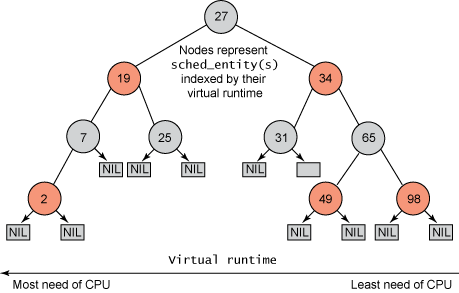
\includegraphics[scale=1]{obrazky/RBT_virtual_runtime.png}
%\caption{Červeno-černý strom úloh setřízený pomocí vruntime}
\caption{RB strom úloh setřízený podle hodnot vruntime}
\label{RB vruntime}
\end{figure}


Aby byl plánovač férový, vezme pro spuštění první úlohu zleva. Čas po který běžela současná úloha, vynásobený koeficientem priority, se přičte k virtuálnímu času běhu a pokud je úloha běžící je vložena zpět do červeno-černého stromu. Úlohám na levé straně stromu je dán čas na procesoru (postupně vždy po jedné úloze) a obsah stromu přebíhá zprava doleva k udržení férovosti. Jednoduše řečeno, všem úlohám je postupně přidělován čas na procesoru (dle pořadí ve stromu zleva doprava) a neustále dochází k vyvažování stromu všech běžících úloh.

\newpage
\subsection{Plánování skupin úloh}

Další velice zajímavou vlastností CFS je koncept plánování skupin úloh. Poprvé implementováno v jádrech 2.6.24. 
Pro přesnější formulaci v této kapitole začneme používat kromě pojmu úloha, která se používá v kontextu jádra, pojem proces a vlákno které jsou z uživatelské terminologie. 

Plánování skupin je nový způsob jak obstarat férovost v plánování, když se proces rozvětví do více vláken. Příkladem tohoto může být HTTP server, který se rozvětví na mnoho vláken za účelem obsluhovat HTTP požadavky paralelně (což je typické pro HTTP servery). Místo aby byly brány všechny vlákna jako úlohy se stejnou váhou, CFS zavádí skupiny, aby takové chování ošetřil. Proces který se větví na vlákna, sdílí jejich vruntime v rámci skupiny a to hierarchicky, zatímco každý další jednotlivý proces (v terminologie jádra úloha) udržuje svůj vlastní vruntime. Tímto způsobem každý další proces dostává přibližně stejné množství plánovaného času jako skupina vláken. V systému můžeme najít \verb#/proc# rozhraní, kterým řídíme hierarchii úloh a které nám dává plnou kontrolu nad tím jak jsou skupiny úloh tvořeny. Pomocí této konfigurace můžeme vytvořit férovost přes uživatele systému, přes úlohy nebo jejich kombinace.

Rozdělování úloh do skupin je v současném jádru automatické. Lze ho zapnou a vypnout v \verb#/proc/sys/kernel/sched_autogroup_enabled#.

\begin{figure}[ht]
\caption{Příklad vytváření skupin multimedia a browser pomocí cgroups}
\center
\label{cgroups}

\begin{Verbatim}[frame=single]

# mount -t tmpfs cgroup_root /sys/fs/cgroup
# mkdir /sys/fs/cgroup/cpu
# mount -t cgroup -ocpu none /sys/fs/cgroup/cpu
# cd /sys/fs/cgroup/cpu

# mkdir multimedia  # vytvorime skupinu uloh multimedia 
# mkdir browser     # vytvorime skupinu uloh multimedia 

# Timto zajistime, ze multimedia budou dostavat 
# 2x vice procesoroveho casu nez skupina browser

# echo 2048 > multimedia/cpu.shares
# echo 1024 > browser/cpu.shares

# firefox &  # Spustime firefox presuneme ho
#            # do skupiny "browser"
# echo <firefox_pid> > browser/tasks

# #spustime gmplayer
# echo <movie_player_pid> > multimedia/tasks

\end{Verbatim}
\end{figure}

\newpage
\subsection{Priority úloh}

CFS nepoužívá fronty úloh pro každou prioritu jak to dělali předchůdci CFS, ale priority jsou řešeny tak, že úlohám s nižší prioritou roste hodnota vruntime rychleji a naopak úlohám s prioritou vyšší roste hodnota vruntime pomaleji.

\subsection{Datové struktury v CFS}

Všechny úlohy jsou v Linuxu reprezentovány strukturou \verb#task_struct#. Tato struktura (spolu s dalšími ze kterých je samotná \verb#task_struct# složená) plně popisují úlohu a zahrnují aktuální stav úlohy, její zásobník, příznaky procesu, prioritu (statickou i dynamickou). Tyto informace a mnohem více podobných struktur lze najít v \verb#include/linux/sched.h#. Z důvodu aby bylo možno plánovat úlohy podle různých pravidel (plánovacích tříd), nenalezneme CFS závislé informace v \verb#task_struct#. Místo toho byla vytvořená nová struktura pojmenovaná \verb#sched_entity# (také z \verb#include/linux/sched.h#) k uchovávání informací o plánování.


\begin{figure}[ht]
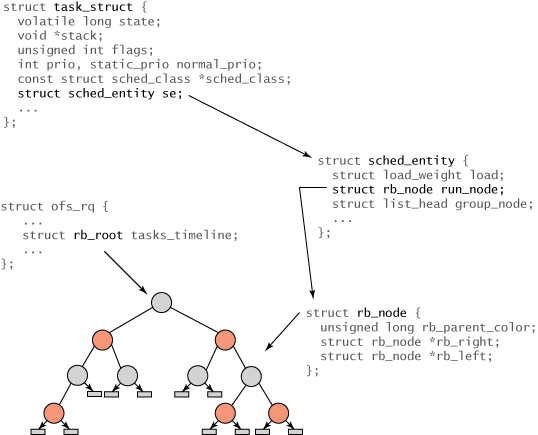
\includegraphics[scale=1]{obrazky/schedulerStructures.png}
\caption{Schéma složení struktur plánovače}
\label{scheduler structures}
\end{figure}


Na kořen stromu je odkazováno pomocí \verb#rb_root# struktury (z \verb#rbtree.h#) ze \verb#cfs_rq# struktury (v \verb#sched.h#).
\verb#cfs_rq# obsahuje také ukazatel na nejvíce levý prvek ve stromu, \verb#min_vruntime#, ukazatele na předchozí a současně běžící úlohu a další informace týkající se skupin a SMP plánování a vyvažování. Samotná priorita procesu je uchována v datové struktuře \verb#load_weight#. 

Uzly RB stromu představují jednu nebo více úloh, které jsou spustitelné. Každý uzel stromu je reprezentován \verb#rb_node# (z \verb#/include/linux/rbtree.h#) strukturou, která neobsahuje nic víc než odkaz na potomka a barvu předka. Entita \verb#rb_node# je součástí \verb#sched_entity# struktury, která zahrnuje \verb#rb_node# odkaz a mnoho různých statistických dat. Nejdůležitější položkou \verb#sched_entity# je vruntime (64bit políčko), která znázorňuje dobu, po kterou proces běžel, a slouží jako index pro červeno-černý strom. Struktura \verb#task_struct# leží na vrcholu hierarchie a plně popisuje úlohu a zahrnuje \verb#sched_entity# strukturu. 

CFS dále udržuje hodnotu \verb#rq->cfs.min_vruntime#, která je monotónně zvyšována na minimální hodnotu vruntime všech úloh ve stromu. Tato hodnota se používá pro umístění nově aktivovaných úloh z nejvíce levé strany stromu.

Celkové množství běžících úloh ve stromu je zaznamenáno v \verb#r->cfs.load# hodnotě, což je suma priorit všech běžících úloh.

\subsection{Aktualizace doby běhu úlohy (vruntime)}

Vstupní funkci k aktualizaci vruntime je \verb#task_tick_fair()# volána z funkce \verb#scheduler_tick# přes odkaz \verb#task_tick()# (z \verb#kernel/sched/core.c#). 

%\begin{lstlisting} 
%
%/*
% * scheduler tick hitting a task of our scheduling class:
% */
%static void task_tick_fair(struct rq *rq, struct task_struct *curr, int queued)
%{
%        struct cfs_rq *cfs_rq;
%        struct sched_entity *se = &curr->se;
%
%        for_each_sched_entity(se) {
%                cfs_rq = cfs_rq_of(se);
%                entity_tick(cfs_rq, se, queued);
%        }
%
%        if (numabalancing_enabled)
%                task_tick_numa(rq, curr);
%
%        update_rq_runnable_avg(rq, 1);
%}
%
%\end{lstlisting} 

Z funkce \verb#task_tick_fair# je volána funkce \verb#entity_tick()#, která dělá dvě věci: 
\begin{enumerate}
\item Aktualizuje vruntime současně běžící úlohy. Toto je realizováno pomocí funkce \verb#update_curr(cfs_rq)#, která  počítá čas strávený úlohou od posledního naplánování (\verb#delta_exec#) a ten je pak použit jako parametr při volání funkce \verb#__update_curr()#, která provede samotnou aktualizaci vruntime. K rozdílu časů běhů je započítána váha priority aktuálně běžící úlohy (váha je uložená v \verb#load_weight#) a výsledek je uložen do vruntime aktuální úlohy. Také dochází ke aktualizaci \verb#min_runtime# hodnoty. 
\item Zjištuje zda je potřeba současně běžící úlohu odebrat. Jakmile je vruntime aktuální úlohy aktualizován, je volána funkce \verb#check_preempt_tick()#. 
\begin{verbatim}
if (cfs_rq->nr_running > 1)
   check_preempt_tick(cfs_rq, curr);
\end{verbatim}
Tato funkce vezme vruntime současné úlohy a kontroluje ji proti vruntime úlohy, která je nejvíce vlevo v červeno-černým stromu, aby zjistil, zda bude nutno aktuálně běžící úlohu vyměnit.
\end{enumerate}

%\begin{lstlisting} 
%
%entity_tick(struct cfs_rq *cfs_rq, struct sched_entity *curr, int queued)
%{
%        /*
%         * Update run-time statistics of the 'current'.
%         */
%        update_curr(cfs_rq);
%        
%        /*
%         * Ensure that runnable average is periodically updated.
%         */
%
%        update_entity_load_avg(curr, 1);
%        update_cfs_rq_blocked_load(cfs_rq, 1);
%        update_cfs_shares(cfs_rq);
%
%#ifdef CONFIG_SCHED_HRTICK
%        /*
%         * queued ticks are scheduled to match the slice, so don't bother
%         * validating it and just reschedule.
%         */
%        if (queued) {
%                resched_curr(rq_of(cfs_rq));
%                return;
%        }
%        /*
%         * don't let the period tick interfere with the hrtick preemption
%         */
%        if (!sched_feat(DOUBLE_TICK) &&
%                        hrtimer_active(&rq_of(cfs_rq)->hrtick_timer))
%                return;
%#endif
%        
%        if (cfs_rq->nr_running > 1)
%                check_preempt_tick(cfs_rq, curr);
%}
%
%
%/*
% * Update the current task's runtime statistics.
% */
%static void update_curr(struct cfs_rq *cfs_rq)
%{
%        struct sched_entity *curr = cfs_rq->curr;
%        u64 now = rq_clock_task(rq_of(cfs_rq));
%        u64 delta_exec;
%
%        if (unlikely(!curr))
%                return;
%
%        delta_exec = now - curr->exec_start;
%        if (unlikely((s64)delta_exec <= 0))
%                return;
%
%        curr->exec_start = now;
%
%        schedstat_set(curr->statistics.exec_max,
%                      max(delta_exec, curr->statistics.exec_max));
%
%        curr->sum_exec_runtime += delta_exec;
%        schedstat_add(cfs_rq, exec_clock, delta_exec);
%
%        curr->vruntime += calc_delta_fair(delta_exec, curr);
%        update_min_vruntime(cfs_rq);
%
%        if (entity_is_task(curr)) {
%                struct task_struct *curtask = task_of(curr);
%
%                trace_sched_stat_runtime(curtask, delta_exec, curr->vruntime);
%                cpuacct_charge(curtask, delta_exec);
%                account_group_exec_runtime(curtask, delta_exec);
%        }
%
%        account_cfs_rq_runtime(cfs_rq, delta_exec);
%}
%
%\end{lstlisting} 

%%%%

Funkce \verb#sched_slice()# volaná z funkce \verb#check_preempt_tick#
\begin{verbatim}
ideal_runtime = sched_slice(cfs_rq, curr);
\end{verbatim}
vrací ideální délku běhu aktuální úlohy v závislosti na množství běžících úloh. 
Jestliže je čas posledního běhu úlohy (delta) větší než tato hodnota, je nastaven na aktuálně běžící úlohu příznak \verb#need_resched#. 
\begin{verbatim}
if (delta_exec > ideal_runtime) {
   resched_curr(rq_of(cfs_rq));
\end{verbatim}
Pokud ne, pak se čas běhu kontroluje proti hodnotě v \verb#min_granularity#. V případě, že úkol běžel déle než \verb#min_granularity# a celkově je na červeno-černém stromě více než jedna úloha provede se porovnání s úlohou nejvíce nalevo v červeno-černém stromu. Jestliže jsou rozdíly mezi časy běhu těchto dvou úloh kladné, pak to znamená, že současná úloha běžela déle než úloha nejvíce nalevo. Dojde také k nastavení \verb#need_resched# příznaku, aby mohlo dojít co nejdřív k přeplánování.
\begin{verbatim} 
if (delta_exec < sysctl_sched_min_granularity)
   return;

se = __pick_first_entity(cfs_rq);
delta = curr->vruntime - se->vruntime;

if (delta < 0)
   return;

if (delta > ideal_runtime)
   resched_curr(rq_of(cfs_rq));
\end{verbatim} 

%\begin{lstlisting} 
%
%/*
% * Preempt the current task with a newly woken task if needed:
% */
%static void
%check_preempt_tick(struct cfs_rq *cfs_rq, struct sched_entity *curr)
%{
%        unsigned long ideal_runtime, delta_exec;
%        struct sched_entity *se;
%        s64 delta;
%
%        ideal_runtime = sched_slice(cfs_rq, curr);
%        delta_exec = curr->sum_exec_runtime - curr->prev_sum_exec_runtime;
%        if (delta_exec > ideal_runtime) {
%                resched_curr(rq_of(cfs_rq));
%                /*
%                 * The current task ran long enough, ensure it doesn't get
%                 * re-elected due to buddy favours.
%                 */
%                clear_buddies(cfs_rq, curr);
%                return;
%        }
%
%        /*
%         * Ensure that a task that missed wakeup preemption by a
%         * narrow margin doesn't have to wait for a full slice.
%         * This also mitigates buddy induced latencies under load.
%         */
%        if (delta_exec < sysctl_sched_min_granularity)
%                return;
%
%        se = __pick_first_entity(cfs_rq);
%        delta = curr->vruntime - se->vruntime;
%
%        if (delta < 0)
%                return;
%
%        if (delta > ideal_runtime)
%                resched_curr(rq_of(cfs_rq));
%}
%
%\end{lstlisting} 
%
%\begin{lstlisting} 
%
%/*
% * We calculate the wall-time slice from the period by taking a part
% * proportional to the weight.
% *
% * s = p*P[w/rw]
% */
%
%static u64 sched_slice(struct cfs_rq *cfs_rq, struct sched_entity *se)
%{
%        u64 slice = __sched_period(cfs_rq->nr_running + !se->on_rq);
%
%        for_each_sched_entity(se) {
%                struct load_weight *load;
%                struct load_weight lw;
%
%                cfs_rq = cfs_rq_of(se);
%                load = &cfs_rq->load;
%
%                if (unlikely(!se->on_rq)) {
%                        lw = cfs_rq->load;
%
%                        update_load_add(&lw, se->load.weight);
%                        load = &lw;
%                }
%                slice = __calc_delta(slice, se->load.weight, load);
%        }
%        return slice;
%}
%
%\end{lstlisting} 

V kostře plánovače jsme se dočetli, jak byly úlohy deaktivovány a vyjmuty z fronty běžících úloh, nebo aktivovaných když se probudily v \verb#try_to_wake_up()#. Ve fair plánovací třídě jsou volány \verb#equeue_task_fair()# a \verb#dequeue_task_fair()# ve funkcích \verb#enqueue_entity()# a \verb#dequeue_entity()# pro aktualizování uzlů v červeno-černém stromu.

%\begin{lstlisting} 
%static void enqueue_entity(struct cfs_rq *cfs_rq, struct sched_entity *se, int flags)
%{
%        /*
%         * Update the normalized vruntime before updating min_vruntime
%         * through calling update_curr().
%         */
%        if (!(flags & ENQUEUE_WAKEUP) || (flags & ENQUEUE_WAKING))
%                se->vruntime += cfs_rq->min_vruntime;
%
%        /*
%         * Update run-time statistics of the 'current'.
%         */
%        update_curr(cfs_rq);
%        enqueue_entity_load_avg(cfs_rq, se, flags & ENQUEUE_WAKEUP);
%        account_entity_enqueue(cfs_rq, se);
%        update_cfs_shares(cfs_rq);
%
%        if (flags & ENQUEUE_WAKEUP) {
%                place_entity(cfs_rq, se, 0);
%                enqueue_sleeper(cfs_rq, se);
%        }
%
%        update_stats_enqueue(cfs_rq, se);
%        check_spread(cfs_rq, se);
%        if (se != cfs_rq->curr)
%                __enqueue_entity(cfs_rq, se);
%        se->on_rq = 1;
%
%        if (cfs_rq->nr_running == 1) {
%                list_add_leaf_cfs_rq(cfs_rq);
%                check_enqueue_throttle(cfs_rq);
%        }
%}
%
%static void dequeue_entity(struct cfs_rq *cfs_rq, struct sched_entity *se, int flags)
%{       
%        /*
%         * Update run-time statistics of the 'current'.
%         */
%        update_curr(cfs_rq);
%        dequeue_entity_load_avg(cfs_rq, se, flags & DEQUEUE_SLEEP);
%        
%        update_stats_dequeue(cfs_rq, se);
%        if (flags & DEQUEUE_SLEEP) {
%#ifdef CONFIG_SCHEDSTATS
%                if (entity_is_task(se)) {
%                        struct task_struct *tsk = task_of(se);
%                        
%                        if (tsk->state & TASK_INTERRUPTIBLE) 
%                                se->statistics.sleep_start = rq_clock(rq_of(cfs_rq));
%                        if (tsk->state & TASK_UNINTERRUPTIBLE)
%                                se->statistics.block_start = rq_clock(rq_of(cfs_rq));
%                }
%#endif  
%        }
%        
%        clear_buddies(cfs_rq, se);
%        
%        if (se != cfs_rq->curr)
%                __dequeue_entity(cfs_rq, se);
%        se->on_rq = 0;
%        account_entity_dequeue(cfs_rq, se);
%        
%        /*
%         * Normalize the entity after updating the min_vruntime because the
%         * update can refer to the ->curr item and we need to reflect this
%         * movement in our normalized position.
%         */
%        if (!(flags & DEQUEUE_SLEEP))
%                se->vruntime -= cfs_rq->min_vruntime;
%        
%        /* return excess runtime on last dequeue */
%        return_cfs_rq_runtime(cfs_rq);
%        
%        update_min_vruntime(cfs_rq);
%        update_cfs_shares(cfs_rq);
%}
%\end{lstlisting} 

Funkce \verb#schedule()# volá funkci \verb#pick_next_task()# určité plánovací třídy s největší prioritou, která má běžící úlohy. Jestliže ve třídě nejsou úlohy, je vrácena hodnota NULL. 
\begin{verbatim} 
do {
        struct sched_entity *curr = cfs_rq->curr;

       if (curr && curr->on_rq)
                update_curr(cfs_rq);
        else
                curr = NULL;

       if (unlikely(check_cfs_rq_runtime(cfs_rq)))
                goto simple;

        se = pick_next_entity(cfs_rq, curr);
        cfs_rq = group_cfs_rq(se);
} while (cfs_rq);
\end{verbatim} 

Z funkce \verb#pick_next_task()# je volána funkce \verb#pick_next_entity()#, která odstraní běžící úlohu z červeno-černého stromu úloh, protože běžící úloha není na stromě obsažena. While smyčka je použita pro počítání férového plánování skupin.

%\begin{lstlisting} 
%static struct task_struct * pick_next_task_fair(struct rq *rq, struct task_struct *prev)
%{
%        struct cfs_rq *cfs_rq = &rq->cfs;
%        struct sched_entity *se;
%        struct task_struct *p;
%        int new_tasks;
%
%again:
%#ifdef CONFIG_FAIR_GROUP_SCHED
%        if (!cfs_rq->nr_running)
%                goto idle;
%
%        if (prev->sched_class != &fair_sched_class)
%                goto simple;
%
%        /*
%         * Because of the set_next_buddy() in dequeue_task_fair() it is rather
%         * likely that a next task is from the same cgroup as the current.
%         *
%         * Therefore attempt to avoid putting and setting the entire cgroup
%         * hierarchy, only change the part that actually changes.
%         */
%
%        do {
%                struct sched_entity *curr = cfs_rq->curr;
%
%                /*
%                 * Since we got here without doing put_prev_entity() we also
%                 * have to consider cfs_rq->curr. If it is still a runnable
%                 * entity, update_curr() will update its vruntime, otherwise
%                 * forget we've ever seen it.
%                 */
%                if (curr && curr->on_rq)
%                        update_curr(cfs_rq);
%                else
%                        curr = NULL;
%
%                /*
%                 * This call to check_cfs_rq_runtime() will do the throttle and
%                 * dequeue its entity in the parent(s). Therefore the 'simple'
%                 * nr_running test will indeed be correct.
%                 */
%                if (unlikely(check_cfs_rq_runtime(cfs_rq)))
%                        goto simple;
%
%                se = pick_next_entity(cfs_rq, curr);
%                cfs_rq = group_cfs_rq(se);
%        } while (cfs_rq);
%
%        p = task_of(se);
%
%        /*
%         * Since we haven't yet done put_prev_entity and if the selected task
%         * is a different task than we started out with, try and touch the
%         * least amount of cfs_rqs.
%         */
%        if (prev != p) {
%                struct sched_entity *pse = &prev->se;
%
%                while (!(cfs_rq = is_same_group(se, pse))) {
%                        int se_depth = se->depth;
%                        int pse_depth = pse->depth;
%
%                        if (se_depth <= pse_depth) {
%                                put_prev_entity(cfs_rq_of(pse), pse);
%                                pse = parent_entity(pse);
%                        }
%                        if (se_depth >= pse_depth) {
%                                set_next_entity(cfs_rq_of(se), se);
%                                se = parent_entity(se);
%                        }
%                }
%
%                put_prev_entity(cfs_rq, pse);
%                set_next_entity(cfs_rq, se);
%        }
%
%        if (hrtick_enabled(rq))
%                hrtick_start_fair(rq, p);
%
%        return p;
%simple:
%        cfs_rq = &rq->cfs;
%#endif
%
%        if (!cfs_rq->nr_running)
%                goto idle;
%
%        put_prev_task(rq, prev);
%
%        do {
%                se = pick_next_entity(cfs_rq, NULL);
%                set_next_entity(cfs_rq, se);
%                cfs_rq = group_cfs_rq(se);
%        } while (cfs_rq);
%
%        p = task_of(se);
%
%        if (hrtick_enabled(rq))
%                hrtick_start_fair(rq, p);
%
%        return p;
%
%idle:
%        new_tasks = idle_balance(rq);
%        /*
%         * Because idle_balance() releases (and re-acquires) rq->lock, it is
%         * possible for any higher priority task to appear. In that case we
%         * must re-start the pick_next_entity() loop.
%         */
%        if (new_tasks < 0)
%                return RETRY_TASK;
%
%        if (new_tasks > 0)
%                goto again;
%
%        return NULL;
%}
%
%\end{lstlisting} 
%
%\begin{lstlisting} 
%
%/*
% * Pick the next process, keeping these things in mind, in this order:
% * 1) keep things fair between processes/task groups
% * 2) pick the "next" process, since someone really wants that to run
% * 3) pick the "last" process, for cache locality
% * 4) do not run the "skip" process, if something else is available
% */
%static struct sched_entity * pick_next_entity(struct cfs_rq *cfs_rq, struct sched_entity *curr)
%{
%        struct sched_entity *left = __pick_first_entity(cfs_rq);
%        struct sched_entity *se;
%
%        /*
%         * If curr is set we have to see if its left of the leftmost entity
%         * still in the tree, provided there was anything in the tree at all.
%         */
%        if (!left || (curr && entity_before(curr, left)))
%                left = curr;
%
%        se = left; /* ideally we run the leftmost entity */
%
%        /*
%         * Avoid running the skip buddy, if running something else can
%         * be done without getting too unfair.
%         */
%        if (cfs_rq->skip == se) {
%                struct sched_entity *second;
%
%                if (se == curr) {
%                        second = __pick_first_entity(cfs_rq);
%                } else {
%                        second = __pick_next_entity(se);
%                        if (!second || (curr && entity_before(curr, second)))
%                                second = curr;
%                }
%
%                if (second && wakeup_preempt_entity(second, left) < 1)

%        }
%
%        /*
%         * Prefer last buddy, try to return the CPU to a preempted task.
%         */
%        if (cfs_rq->last && wakeup_preempt_entity(cfs_rq->last, left) < 1)
%                se = cfs_rq->last;
%
%        /*
%         * Someone really wants this to run. If it's not unfair, run it.
%         */
%
%        if (cfs_rq->next && wakeup_preempt_entity(cfs_rq->next, left) < 1)
%                se = cfs_rq->next;
%
%        clear_buddies(cfs_rq, se);
%
%        return se;
%}
%
%\end{lstlisting} 

\subsection{Shrnutí}

CFS je volán v době když dojde k vytvoření nové úlohy či probuzení stávající úlohy, usnutí úlohy, nebo když je vyvoláno jako obsluha časovače přerušení. Spočítá čas právě strávený úlohou na CPU, vynásobí ho koeficientem priority úlohy a přičte jej do \verb#p->se.vruntime#. Jestliže \verb#p->se.vruntime# poroste dostatečně a současně běžící úloha již není úlohou s nejmenší hodnotou vruntime, pak je spuštěna úloha, která je nejvíce nalevo v červeno-černého stromu. Úloha která právě běžela se vrátí zpátky do stromu. Toto není úplně přesné, jelikož CFS má nastavenou hodnotu granularity, o kterou maximálně může být větší vruntime běžící úlohy než vruntime úlohy úplně nalevo ve stromu. S granuralitou se počítá proto, aby z důvodu velmi malého rozdílu v hodnotě vruntime mezi úlohami nedocházelo k výměně obsahu a s tím souvisejícím negativním jevům jako zahozením dat ve vyrovnávací paměti atd.
V systému jde granularitu konfigurovat \newline v \verb#/proc/sys/kernel/sched_min_granularity_ns#. 

Zmenšením hodnoty v \verb#sched_min_granularity_ns# docílíme k rychlejší odezvě a k menší propustnosti (z důvodu častější výměny obsahu). Zvýšení hodnoty bude vést k větší propustnosti, ale bude mít pomalejší odezvu na interaktivní procesy (vhodné pro servery). 

Větší část CFS návrhu už je mimo tento jednoduchý koncept, přibyly zde rozšíření pro vyvažování úloh na NUMA systémech a dalších algoritmy například na rozpoznávání spících procesů.

\section{Vyvažování}

\subsection{Vyvažování na UMA SMP systémech}

UMA – uniform memory access. Znamená, že přístup jakéhokoli procesoru do jakéhokoli segmentu paměti je vždy stejně rychlý.

Vyvažování na SMP systémech bylo implementováno s cílem zlepšit výkonnost tím, že odebereme úlohy od nejvíce vytížených CPU a přesuneme je na CPU volné nebo méně vytížené. Linuxový plánovač kontroluje pravidelně, jak jsou rozmístěné úlohy na systému a když vidí, že systém není vyvážen, spustí vyvažování.

Důležitým bodem je správné chápání topologie systému plánovačem. Můžeme mít systémy s několika jádry, kde mohou úlohy trpět více vyprázdněním vyrovnávacích pamětí v důsledku přesunu úloh, než v důsledku běhu úlohy na vytíženém CPU. Jiné systémy zase mohou být více flexibilní vůči migraci úloh a to díky sdíleným vyrovnávacím pamětem (například systémy podporující hyperthreading).

Kvůli rozdílům v topologiích systémů, byly zavedeny od jádra 2.6 plánovací domény. Plánovací domény vytváří hierarchické skupiny procesorů v systému, které poskytují jádru OS přehled o topologii systému a usnadňují vyvažování.

\newpage
\subsubsection{Plánovací domény a skupiny}

Plánovací doména je množina procesorů, které sdílejí vlastnosti a plánování pravidla, která mohou být vyvažovány mezi sebou. Každá doména může obsahovat jednu nebo více plánovacích skupin, které se považují za jednotku v doméně. Takže když se plánovač snaží vyvážit zatížení v rámci domény, pokusí se vyvážit zatížení každé plánovací skupiny, bez ohledu na to co se děje ve skupině.



Představme si, že máme systém dvou fyzických procesorů, na kterých je hyperthreading\footnote{Hyper Threading funguje na principu duplikace té části CPU, která obsahuje registry, což pro aplikace vyvolává dojem, že procesorů je vícero a zasílají pro zpracování procesorem víc instrukcí a příkazů naráz.}, tak dostaneme celkem čtyři logické procesory. Při spuštění systému, jádro rozdělí logické jádra do doménové hierarchie druhé úrovně viz obrázek \ref{domeny a skupiny}.

\begin{figure}[ht]
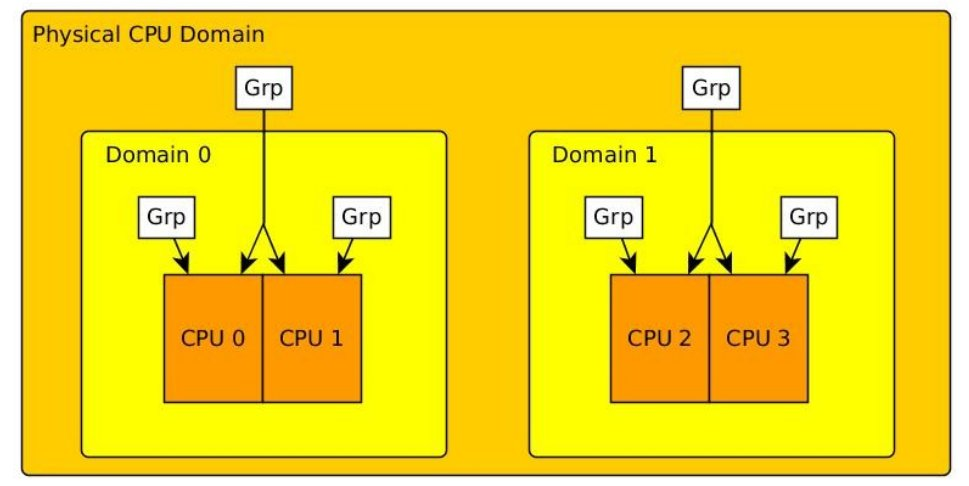
\includegraphics[scale=0.53]{obrazky/domenyAskupiny.jpeg}
\caption{Schéma skupin a domén}
\label{domeny a skupiny}
\end{figure}

Každý hyperthreadový procesor je vložen právě do jedné skupiny a obě skupiny jsou v téže doméně. Tyto dvě úrovně domén poté tvoří celý procesor. 

%Diagram pro NUMA systémy je stejný jako předchozí diagram. Jednotlivé domény pak reprezentují NUMA nody. 

%\subsection{Vyvažování zátěže}

Každá plánovací doména má vyvažovací pravidla, která jsou platná pouze na této úrovni (tzn. v této doméně). 

Parametry pravidel zahrnují, jak často se máme pokusit udělat vyvážení napříč doménou, jaké je povoleno mít nevyvážené zatížení mezi skupinami procesorů, než se spustí vyvažování, jak moc je povoleno mít nevyvážené zatížení na procesoru, než se spustí vyvažování, jak dlouho může být úloha mimo procesor, než považujeme její vyrovnávací paměť za ztracenou.
Existují také příznaky, které nám signalizují změny v zatížení systému. 

Aktivní vyvažování zátěže je spouštěno pravidelně. Dochází k procházení hierarchie domén nahoru a zjišťuje se, zdali jsou všechny skupiny po cestě vyvážené. Když se narazí na nějakou nevyváženou, provádí vyvažování podle pravidel dané domény.

\newpage
\subsubsection{Implementace vyvažování}

Ve \verb#sched.h# najdeme dvě struktury, které byly přidány do kódu za účelem vyvažování. Jedná se o \verb#sched_domain# (\verb#include/linux/sched.h#) a pak \verb#sched_group# (\verb#kernel/sched/sched.h#).

\begin{verbatim} 

struct sched_domain {
        /* These fields must be setup */
        struct sched_domain *parent;
        struct sched_domain *child;
        struct sched_group *groups;

                	...

\end{verbatim} 


%        /* Runtime fields. */
%        unsigned long last_balance;     /* init to jiffies. units in jiffies */
%        unsigned int balance_interval;  /* initialise to 1. units in ms. */
%        unsigned int nr_balance_failed; /* initialise to 0 */
%
%        /* idle_balance() stats */
%        u64 max_newidle_lb_cost;
%        unsigned long next_decay_max_lb_cost;
%
%#ifdef CONFIG_SCHEDSTATS
%        /* load_balance() stats */
%        unsigned int lb_count[CPU_MAX_IDLE_TYPES];
%        unsigned int lb_failed[CPU_MAX_IDLE_TYPES];
%        unsigned int lb_balanced[CPU_MAX_IDLE_TYPES];
%        unsigned int lb_imbalance[CPU_MAX_IDLE_TYPES];
%        unsigned int lb_gained[CPU_MAX_IDLE_TYPES];
%        unsigned int lb_hot_gained[CPU_MAX_IDLE_TYPES];
%        unsigned int lb_nobusyg[CPU_MAX_IDLE_TYPES];
%        unsigned int lb_nobusyq[CPU_MAX_IDLE_TYPES];
%
%        /* Active load balancing */
%        unsigned int alb_count;
%        unsigned int alb_failed;
%
%        unsigned int alb_pushed;
%
%        /* SD_BALANCE_EXEC stats */
%        unsigned int sbe_count;
%        unsigned int sbe_balanced;
%        unsigned int sbe_pushed;
%
%        /* SD_BALANCE_FORK stats */
%        unsigned int sbf_count;
%        unsigned int sbf_balanced;
%        unsigned int sbf_pushed;
%
%        /* try_to_wake_up() stats */
%        unsigned int ttwu_wake_remote;
%        unsigned int ttwu_move_affine;
%        unsigned int ttwu_move_balance;
%#endif
%#ifdef CONFIG_SCHED_DEBUG
%        char *name;
%#endif
%        union {
%                void *private;          /* used during construction */
%                struct rcu_head rcu;    /* used during destruction */
%        };
%
%        unsigned int span_weight;
%        /*
%         * Span of all CPUs in this domain.
%         *
%         * NOTE: this field is variable length. (Allocated dynamically
%         * by attaching extra space to the end of the structure,
%         * depending on how many CPUs the kernel has booted up with)
%         */
%        unsigned long span[0];
%};

\begin{verbatim} 

struct sched_group {
        struct sched_group *next;
        atomic_t ref;

        unsigned int group_weight;
        struct sched_group_capacity *sgc;

        unsigned long cpumask[0];
};

\end{verbatim} 

V \verb#include/linux/topology.h# najdeme nastavení pro příznaky a pro plánovací domény. V \verb#sched_group# můžeme najít strukturu \verb#sgc#, která vyjadřuje \verb#sched_group_capacity#. Vyjadřuje výpočetní sílu dané skupiny. Například dva procesory budou mít hodnotu někde kolem 2, ale CPU s hyperthreadingem bude mít sílu jen kolem 1.1. 

\subsubsection{Aktivní vyvažování}

Během aktivního vyvažování jádro prochází doménovou hierarchií. Začíná se na CPU doméně a postupuje výše. Když na určité doméně zjistí, že je nevyvážená, spustí vyvažovací operace.

Během inicializace plánovače je vytvořena obsluha pravidelného přerušení, ze které jsou volány funkce, které provádí vyvažování zátěže. Vyvažování je spuštěno ve funkci \verb#scheduler_tick()# (\verb#kernel/sched/core.c#) voláním \linebreak \verb#trigger_load_balance()# (\verb#kernel/sched/fair.c#). 

\verb#trigger_load_balance()# zkontroluje časovač a jestli je vyvažování potřeba spustí obsluhu softwarového přerušení \verb#SCHED_SOFTIRQ#.

\newpage
\begin{verbatim} 
void trigger_load_balance(struct rq *rq)
{
   if (unlikely(on_null_domain(rq)))
      return;

   if (time_after_eq(jiffies, rq->next_balance))
      raise_softirq(SCHED_SOFTIRQ);
   #ifdef CONFIG_NO_HZ_COMMON
      if (nohz_kick_needed(rq))
         nohz_balancer_kick();
   #endif
}
\end{verbatim} 

Výjimka je obsloužena funkcí \verb#run_rebalance_domains()#, která volá \linebreak \verb#rebalance_domains()#. 

\begin{verbatim} 

static void run_rebalance_domains(struct softirq_action *h)
{
   struct rq *this_rq = this_rq();
   enum cpu_idle_type idle = this_rq->idle_balance ?
                              CPU_IDLE : CPU_NOT_IDLE;

   rebalance_domains(this_rq, idle);
   nohz_idle_balance(this_rq, idle);
}

\end{verbatim} 

Funkce \verb#rebalance_domains()# poté prochází doménovou hierarchii a volá \verb#load_balance()#, pokud má daná doména nastavenou proměnnou \linebreak \verb#SD_LOAD_BALANCE# a vypršel již interval indikující stav vyvážení. Vyvažovací interval \footnote{počítadlo času počítající čas k dalšímu spuštění vyvažování domén} domény je ve vteřinách a je aktualizován po každém běhu vyvažování.

Aktivní vyvažování je o přetažení jedné nebo více úloh z přetíženého CPU na jiné méně vytížené CPU. Nedochází k výměně úloh, ale pouze k přesunu úlohy. Funkce, která provádí přesun úlohy na jiné CPU, se nazývá \verb#load_balance()#. Jestliže najde nevyváženou skupinu, přesouvá jednu nebo více úloh na současné CPU a vrací hodnotu větší než 0.

%\begin{lstlisting} 
%
%/*
% * Check this_cpu to ensure it is balanced within domain. Attempt to move
% * tasks if there is an imbalance.
% */
%static int load_balance(int this_cpu, struct rq *this_rq,
	%			struct sched_domain *sd, enum cpu_idle_type idle,
%			int *continue_balancing)
%{
%	int ld_moved, cur_ld_moved, active_balance = 0;
%	struct sched_domain *sd_parent = sd->parent;
%	struct sched_group *group;
%	struct rq *busiest;
%	unsigned long flags;
%	struct cpumask *cpus = this_cpu_cpumask_var_ptr(load_balance_mask);
%
%	struct lb_env env = {
%		.sd		= sd,
%		.dst_cpu	= this_cpu,
%		.dst_rq		= this_rq,
%		.dst_grpmask    = sched_group_cpus(sd->groups),
%		.idle		= idle,
%		.loop_break	= sched_nr_migrate_break,
%		.cpus		= cpus,
%		.fbq_type	= all,
%		.tasks		= LIST_HEAD_INIT(env.tasks),
%	};
%
%	/*
%	 * For NEWLY_IDLE load_balancing, we don't need to consider
%	 * other cpus in our group
%	 */
%	if (idle == CPU_NEWLY_IDLE)
%		env.dst_grpmask = NULL;
%
%	cpumask_copy(cpus, cpu_active_mask);
%
%	schedstat_inc(sd, lb_count[idle]);
%
%redo:
%	if (!should_we_balance(&env)) {
%		*continue_balancing = 0;
%		goto out_balanced;
%	}
%
%	group = find_busiest_group(&env);
%	if (!group) {
%		schedstat_inc(sd, lb_nobusyg[idle]);
%		goto out_balanced;
%	}
%
%	busiest = find_busiest_queue(&env, group);
%	if (!busiest) {
%		schedstat_inc(sd, lb_nobusyq[idle]);
%		goto out_balanced;
%	}
%
%<- Zde je pro nas nepodstatna cast kodu ->
%
%	goto out;
%
%out_balanced:
%	/*
%	 * We reach balance although we may have faced some affinity
%	 * constraints. Clear the imbalance flag if it was set.
%	 */
%	if (sd_parent) {
%		int *group_imbalance = &sd_parent->groups->sgc->imbalance;
%
%		if (*group_imbalance)
%			*group_imbalance = 0;
%	}
%
%out_all_pinned:
%	/*
%	 * We reach balance because all tasks are pinned at this level so
%	 * we can't migrate them. Let the imbalance flag set so parent level
%	 * can try to migrate them.
%	 */
%	schedstat_inc(sd, lb_balanced[idle]);
%
%	sd->nr_balance_failed = 0;
%
%out_one_pinned:
%	/* tune up the balancing interval */
%	if (((env.flags & LBF_ALL_PINNED) &&
%			sd->balance_interval < MAX_PINNED_INTERVAL) ||
%			(sd->balance_interval < sd->max_interval))
%		sd->balance_interval *= 2;
%
%	ld_moved = 0;
%out:
%	return ld_moved;
%}
%
%\end{lstlisting} 

Funkce \verb#load_balance()# volá funkci \verb#find_busiest_group()#, která hledá nevyváženost v dané \verb#sched_domain# a vrací nejvíce zatíženou skupinu pokud taková existuje. Jestliže je systém vyvážený a žádná skupina nebyla nalezena, funkce \verb#load_balance()# skončí.

Jestliže funkce \verb#find_busiest_group# vrátila nejvytíženější skupinu, pak ta je předána do funkce \verb#find_busiest_queue()# a výstupem z funkce je fronta úloh nejvíce zatíženého logického procesoru ve skupině.

\verb#load_balance()# poté hledá úlohu v běžící frontě úloh, kterou přesune na frontu současného procesoru voláním \verb#move_tasks()#. Množství úloh, které mají být přesunuty jsou specifikovány jako parametr ve funkci \newline \verb#find_busiest_group()#. Běžně se stává, že všechny úlohy není vhodné přesouvat na jiné CPU a to kvůli vyrovnávací paměti na CPU na kterém předtím běžely. V tomto případě funkce \verb#load_balance# pokračuje v hledání, ale vynechá předchozí nalezené CPU.

Pokud je proměnná \verb#SD_POWERSAVINGS_BALANCE# nastavena v doménových pravidlech a není-li nalezena nejrušnější skupina, \verb#find_busiest_group()# hledá nejméně vytíženou skupinu v \verb#sched_domain#. Procesory z této skupiny jsou poté uvedeny do klidového stavu. 

%\begin{lstlisting} 
%
%/*
% * It checks each scheduling domain to see if it is due to be balanced,
% * and initiates a balancing operation if so.
% *
% * Balancing parameters are set up in init_sched_domains.
% */
%static void rebalance_domains(struct rq *rq, enum cpu_idle_type idle)
%{
%        int continue_balancing = 1;
%        int cpu = rq->cpu;
%        unsigned long interval;
%        struct sched_domain *sd;
%        /* Earliest time when we have to do rebalance again */
%        unsigned long next_balance = jiffies + 60*HZ;
%        int update_next_balance = 0;
%        int need_serialize, need_decay = 0;
%        u64 max_cost = 0;
%
%        update_blocked_averages(cpu);
%
%        rcu_read_lock();
%        for_each_domain(cpu, sd) {
%                /*
%                 * Decay the newidle max times here because this is a regular
%                 * visit to all the domains. Decay ~1% per second.
%                 */
%                if (time_after(jiffies, sd->next_decay_max_lb_cost)) {
%                        sd->max_newidle_lb_cost =
%                                (sd->max_newidle_lb_cost * 253) / 256;
%                        sd->next_decay_max_lb_cost = jiffies + HZ;
%                        need_decay = 1;
%                }
%                max_cost += sd->max_newidle_lb_cost;
%
%                if (!(sd->flags & SD_LOAD_BALANCE))
%                        continue;
%
%                /*
%                 * Stop the load balance at this level. There is another
%                 * CPU in our sched group which is doing load balancing more
%                 * actively.
%                 */
%                if (!continue_balancing) {
%                        if (need_decay)
%                                continue;
%                        break;
%                }
%
%                interval = get_sd_balance_interval(sd, idle != CPU_IDLE);
%
%
%                need_serialize = sd->flags & SD_SERIALIZE;
%                if (need_serialize) {
%                        if (!spin_trylock(&balancing))
%                                goto out;
%                }
%
%                if (time_after_eq(jiffies, sd->last_balance + interval)) {
%                        if (load_balance(cpu, rq, sd, idle, &continue_balancing)) {
%                                /*
%                                 * The LBF_DST_PINNED logic could have changed
%                                 * env->dst_cpu, so we can't know our idle
%                                 * state even if we migrated tasks. Update it.
%                                 */
%                                idle = idle_cpu(cpu) ? CPU_IDLE : CPU_NOT_IDLE;
%                        }
%                        sd->last_balance = jiffies;
%                        interval = get_sd_balance_interval(sd, idle != CPU_IDLE);
%                }
%                if (need_serialize)
%                        spin_unlock(&balancing);
%out:
%                if (time_after(next_balance, sd->last_balance + interval)) {
%                        next_balance = sd->last_balance + interval;
%                        update_next_balance = 1;
%                }
%        }
%        if (need_decay) {
%                /*
%                 * Ensure the rq-wide value also decays but keep it at a
%                 * reasonable floor to avoid funnies with rq->avg_idle.
%                 */
%                rq->max_idle_balance_cost =
%                        max((u64)sysctl_sched_migration_cost, max_cost);
%        }
%        rcu_read_unlock();
%
%        /*
%         * next_balance will be updated only when there is a need.
%         * When the cpu is attached to null domain for ex, it will not be
%         * updated.
%         */
%        if (likely(update_next_balance))
%                rq->next_balance = next_balance;
%}
%
%\end{lstlisting} 

\subsubsection{Vyvažování nečinnosti}
\vbox{%

Vyvažování nečinnosti začíná, když se CPU stává nečinným. Je volána funkce schedule() na CPU vykonávající současnou úlohu, jestliže se jeho fronta běžících úloh vyprázdnila.

Tak jako aktivní vyvažování je i vyvažování nečinnosti \verb#idle_balance()# implementováno v souboru fair.c. Kontroluje se, zdali je průměrná doba čekání ve frontě nečinnosti větší než je cena migrace úlohy na tuto frontu. To znamená, že se kontroluje zdali má cenu vzít úlohu odjinud, nebo jestli je lepší jen počkat, jelikož je pravděpodobné, že se další úloha brzy probudí. Pokud migrace úlohy dává smysl, \verb#idle_balance()# funguje téměř jako \verb#rebalance_domains()#. To projde doménovou hierarchii a volá \verb#idle_balance()# pro domény, které mají v doméně nastaveny příznaky \verb#SD_LOAD_BALANCE# a \verb#SD_BALANCE_NEWIDLE#.}


%\begin{lstlisting} 
%
%/*
% * idle_balance is called by schedule() if this_cpu is about to become
% * idle. Attempts to pull tasks from other CPUs.
% */
%static int idle_balance(struct rq *this_rq)
%{
%        unsigned long next_balance = jiffies + HZ;
%        int this_cpu = this_rq->cpu;
%        struct sched_domain *sd;
%        int pulled_task = 0;
%        u64 curr_cost = 0;
%
%        idle_enter_fair(this_rq);
%
%        /*
%         * We must set idle_stamp _before_ calling idle_balance(), such that we
%         * measure the duration of idle_balance() as idle time.
%         */
%        this_rq->idle_stamp = rq_clock(this_rq);
%
%        if (this_rq->avg_idle < sysctl_sched_migration_cost ||
%            !this_rq->rd->overload) {
%                rcu_read_lock();
%                sd = rcu_dereference_check_sched_domain(this_rq->sd);
%                if (sd)
%                        update_next_balance(sd, 0, &next_balance);
%                rcu_read_unlock();
%
%                goto out;
%        }
%
%        /*
%         * Drop the rq->lock, but keep IRQ/preempt disabled.
%         */
%        raw_spin_unlock(&this_rq->lock);
%
%        update_blocked_averages(this_cpu);
%        rcu_read_lock();
%        for_each_domain(this_cpu, sd) {
%                int continue_balancing = 1;
%                u64 t0, domain_cost;
%
%                if (!(sd->flags & SD_LOAD_BALANCE))
%                        continue;
%
%                if (this_rq->avg_idle < curr_cost + sd->max_newidle_lb_cost) {
%                        update_next_balance(sd, 0, &next_balance);
%                        break;
%                }
%
%                if (sd->flags & SD_BALANCE_NEWIDLE) {
%
%                      t0 = sched_clock_cpu(this_cpu);
%
%                        pulled_task = load_balance(this_cpu, this_rq,
%                                                   sd, CPU_NEWLY_IDLE,
%                                                   &continue_balancing);
%
%                        domain_cost = sched_clock_cpu(this_cpu) - t0;
%                        if (domain_cost > sd->max_newidle_lb_cost)
%                                sd->max_newidle_lb_cost = domain_cost;
%
%                        curr_cost += domain_cost;
%                }
%
%                update_next_balance(sd, 0, &next_balance);
%
%                /*
%                 * Stop searching for tasks to pull if there are
%                 * now runnable tasks on this rq.
%                 */
%                if (pulled_task || this_rq->nr_running > 0)
%                        break;
%        }
%        rcu_read_unlock();
%
%        raw_spin_lock(&this_rq->lock);
%
%        if (curr_cost > this_rq->max_idle_balance_cost)
%                this_rq->max_idle_balance_cost = curr_cost;
%
%        /*
%         * While browsing the domains, we released the rq lock, a task could
%         * have been enqueued in the meantime. Since we're not going idle,
%         * pretend we pulled a task.
%         */
%        if (this_rq->cfs.h_nr_running && !pulled_task)
%                pulled_task = 1;
%
%out:
%        /* Move the next balance forward */
%        if (time_after(this_rq->next_balance, next_balance))
%                this_rq->next_balance = next_balance;
%
%        /* Is there a task of a high priority class? */
%        if (this_rq->nr_running != this_rq->cfs.h_nr_running)
%                pulled_task = -1;
%
%        if (pulled_task) {
%                idle_exit_fair(this_rq);
%                this_rq->idle_stamp = 0;
%        }
%
%        return pulled_task;
%}
%
%\end{lstlisting} 


\subsubsection{Výběr fronty pro novou úlohu}

Dále je třeba dělat vyvažování, když se úloha probudí, nebo je vytvořená nová a potřebuje být umístěná ve frontě běžících úloh. Tato fronta musí být vybrána s ohledem na vyvážení úlohami celého systému. Každá plánovací třída implementuje svojí vlastní strategii na nakládání se svými úlohami a poskytuje funkce \verb#select_task_rq()#, která je volána plánovačem během spuštění úlohy. Je volána ze třech různých důvodů, které jsou vyznačeny pomocí návěští odpovídající domény.

\begin{enumerate}

\item \verb#SD_BALANCE_EXEC# je návěští používané funkci \verb#sched_exec()#. Tato funkce je volána, jestliže úloha startuje jako nová systémovým voláním exec(). Nová úloha je jednoduchá pro vyvažování (neřešíme afinitu vyrovnávací paměti apod).
\item \verb#SD_BALANCE_FORK# je návěští používané ve funkci \verb#wake_up_new_task()#. Tato funkce je volána, když je vytvořená úloha probuzena první krát.
\item \verb#SD_BALANCE_WAKE# je návěští používané ve funkci  \verb#try_to_wake_up()#. Toto je nejsložitější případ, jelikož úloha která běžela předtím, má určitou afinitu vyrovnávací paměti. Proto je třeba vybrat frontu na které budeme mít dostupnou vyrovnávací paměť.

\end{enumerate}

\newpage
\subsection{Numa vyvažování}

NUMA je zkratka non uniform memory access. Systémy založené na této architektuře mají přístupy do různých segmentů paměti je různě rychlé. Architektura je rozšířením SMP (symetrický multi processing). V době kdy se začaly objevovat systémy se stovkami jader, začaly mít počítače problémy s propustností mezi pamětí a procesorem, jelikož každé jádro komunikovalo stejnou sběrnicí s pamětí. Toto se podařilo vyřešit shlukováním jader a pamětí do takzvaných NUMA uzlů. Každý procesor (několik jader) má k dispozici svou lokální paměť, na kterou má rychlý přístup, ale má také přístup na vzdálenou paměť, kde je přístup pomalejší. NUMA systémy lze nalézt na architekturách x86 a ppc. NUMA topologie se používá na serverových systémech s větším počtem CPU socketu v systému.

K propojování uzlů je použita sběrnice, které se obecně říká INTERCONNECT. Každý z výrobců NUMA systémů pojmenovává tyto sběrnice jinak INTEL používá Intel Quick Path (QPI), dříve taky používal název Common system interface (CSI), AMD používá název Hypertransport.

Výrobci systémů si sami navrhují, které NUMA uzly budou propojeny pomoci interconnect sběrnice na přímo, některé další jsou propojeny přes několik dalších NUMA uzlů. 

%h v místě výskytu (here)
%t na začátku stránky (top)
%b na konci stránky (bottom)
%p na samostatné stránce (page of oats)

\begin{figure}[ht]
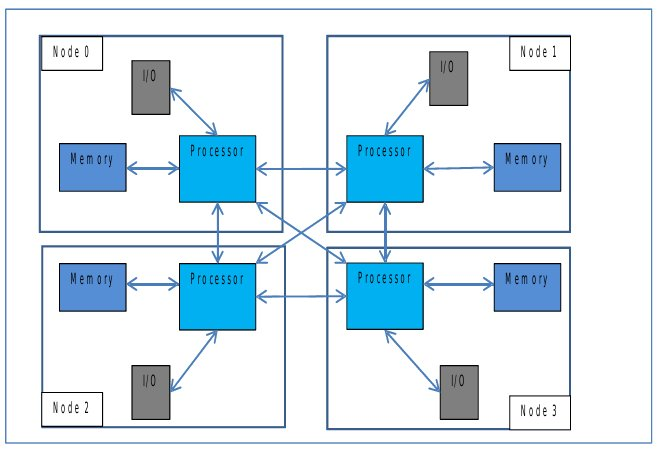
\includegraphics[scale=0.78]{obrazky/numa-scheme.jpeg}
\caption{Jednoduchá NUMA topologie}
\label{numa scheme1}
\end{figure}

obrázek \ref{numa scheme1} ukazuje NUMA topologii systému HP PROLIANT DL580 GEN8 4 socket Ivy Bridge EX processor. Je to nejjednodušší způsob zapojení NUMA počítače. Všechny procesory mají přístup ke své lokální paměti (což je vždy stejné), ale navíc jsou propojeny pomocí QPI s každým dalším NUMA uzlem. Z čehož nám vyplývá, že systém bude mít pouze 2 různé doby přístupu do pamětí. Lokální které jsou nejrychlejší a vzdálené, které jsou pomalejší, ale mezi každými dvěmi uzly vždy stejné.

Zde je výpis numactl ukazující jak máme shlukovány jádra a paměť do NUMA uzlů.

\begin{verbatim} 

# numactl -H
available: 4 nodes (0-3)
node 0 cpus: 0 1 2 3 4 5 6 7 8 9 10 11 12 13 14
node 0 size: 262040 MB
node 0 free: 249261 MB
node 1 cpus: 15 16 17 18 19 20 21 22 23 24 25 26 27 28 29
node 1 size: 262144 MB
node 1 free: 252060 MB
node 2 cpus: 30 31 32 33 34 35 36 37 38 39 40 41 42 43 44
node 2 size: 262144 MB
node 2 free: 250441 MB
node 3 cpus: 45 46 47 48 49 50 51 52 53 54 55 56 57 58 59
node 3 size: 262144 MB
node 3 free: 250080 MB

\end{verbatim}

Následuje tabulka ukazující jak vzdálené (a tím i rychlé) jsou přístupy do paměti.

\begin{verbatim}

node distances:
node 0 1 2 3
0: 10 21 21 21
1: 21 10 21 21
2: 21 21 10 21
3: 21 21 21 10

\end{verbatim}

Na diagonále je vidět čas lokálního přístupu do paměti. Na zbylé uzly přistupujeme vždy stejně kvalitní a dlouhou linkou QPI, takže časy jsou stejné.

Takto symetrický přístup k vzdáleným NUMA pamětem je méně častý. Většina velkých systémů má topologii složitější, kde jsou propojovány uzly přes kontroléry a ty jsou pak přes další kontrolér propojené s dalšími uzly. Dochází tak k přístupům do vzdálené paměti přes více NUMA uzlů a tím pádem dochází k pomalejšímu přístupu do vzdálené paměti. Teď se podívejme na obrázek \ref{numa scheme2} na kterém je systém, který má NUMA topologii složitější. Jde o systém se čtyřmi Westmere procesory HP Proliant DL980 G78.

\begin{figure}[ht]
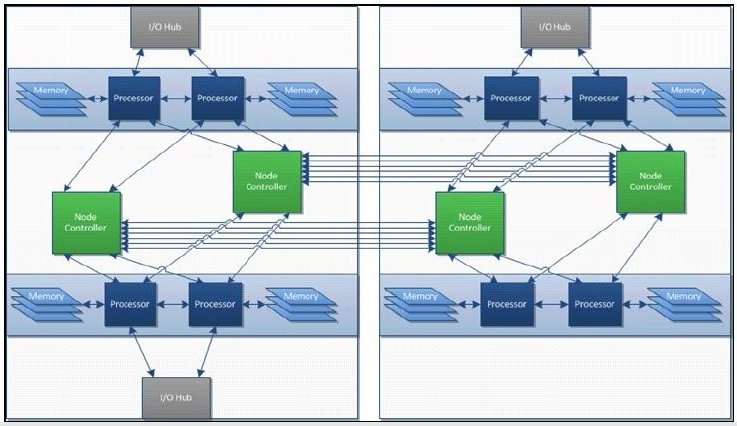
\includegraphics[scale=0.7]{obrazky/numa-scheme-big-system.jpeg}
\caption{Systém se složitější NUMA topologii}
\label{numa scheme2}
\end{figure}


Jedná se o systém s 80 logickými jádry (s 40 fyzickými) a se zapnutou podporou hypertheading. Každý procesor této generace obsahuje 10 logických jader (5 fyzických). Každý procesor se svou lokální pamětí tvoří jeden NUMA uzel. CPU jsou po čtyřech spojené s jedním CPU kontrolérem. Ten je spojuje se zbylými 4 CPU přes další CPU kontrolér. Ze samotného obrázku je vidět, že nyní nebudou přístupy do pamětí dvojího druhu lokální a vzdálené, ale vzdálené se nám dále budou lišit podle toho, přes kolik kontrolérů bude uzel přistupovat k paměti (1 nebo 2). Takže vidíme, že přístupy do pamětí budou dle Obrázku \ref{numa scheme2} čtyř druhů. První je lokální, druhý vzdálený jen mezi uzly vedle sebe (bez využití kontroléru), třetí je vzdálený komunikující přes jeden kontrolér, čtvrtý je vzdálený komunikující přes 2 kontroléry. Z Obrázku \ref{numa scheme2} je patrné, že je cesta mezi NUMA uzly, které jdou přes 2 kontroléry zdvojená tj. existuje zde alternativní cesta pro případ, že bude daná cesta přetížená. To která cesta bude vybrána v případě přístupu do vzdálené paměti přes dva kontroléry rozhoduje firmware kontroléru, takže tímto se dále nemusíme zabývat a bereme to, že je vždy vybrána méně zatížená cesta.

\newpage
Vypíšeme si nejdříve jak jsou jednotlivé jádra shlukovány do uzlů a poté se podíváme, jak se liší vzdálené přístupy do pamětí.

\begin{verbatim}

# numactl -H
available: 8 nodes (0-7)
node 0 cpus: 0 1 2 3 4 5 6 7 8 9
node 0 size: 262133 MB
node 0 free: 250463 MB
node 1 cpus: 10 11 12 13 14 15 16 17 18 19
node 1 size: 262144 MB
node 1 free: 256316 MB
node 2 cpus: 20 21 22 23 24 25 26 27 28 29
node 2 size: 262144 MB
node 2 free: 256439 MB
node 3 cpus: 30 31 32 33 34 35 36 37 38 39
node 3 size: 262144 MB
node 3 free: 255403 MB
node 4 cpus: 40 41 42 43 44 45 46 47 48 49
node 4 size: 262144 MB
node 4 free: 256546 MB
node 5 cpus: 50 51 52 53 54 55 56 57 58 59
node 5 size: 262144 MB
node 5 free: 256036 MB
node 6 cpus: 60 61 62 63 64 65 66 67 68 69
node 6 size: 262144 MB
node 6 free: 256468 MB
node 7 cpus: 70 71 72 73 74 75 76 77 78 79
node 7 size: 262144 MB
node 7 free: 255232 MB

\end{verbatim}

\newpage
\noindent
A nyní se podíváme na přístupy do paměti mezi jednotlivými NUMA uzly. 
\begin{verbatim}

node distances:
node 0 1 2 3 4 5 6 7
0: 10 12 17 17 19 19 19 19
1: 12 10 17 17 19 19 19 19
2: 17 17 10 12 19 19 19 19
3: 17 17 12 10 19 19 19 19
4: 19 19 19 19 10 12 17 17
5: 19 19 19 19 12 10 17 17
6: 19 19 19 19 17 17 10 12
7: 19 19 19 19 17 17 12 10

\end{verbatim}
\noindent
Nyní přístupy do paměti nabývají těchto hodnot:
\begin{enumerate}
\item Hodnoty 10 nejlepšího tedy nejnižšího času jsme dosáhli při přístupu do lokální paměti.
\item Hodnoty 12 druhého nejlepšího času přístupu jsme dosáhli při přístupu na vedlejší uzel, bez potřeby komunikovat přes NUMA kontrolér. 
\item Třetí hodnoty jsme dosáhli při přístupu na vzdálený uzel, který komunikuje přes jeden kontrolér.
\item Nejhorší možný čas přístupu do paměti jsme dosáhli v případě, že komunikují dva NUMA uzly, které jsou propojeny pomocí dvou kontrolérů.
\end{enumerate}

\noindent
Na NUMA systému dochází k těmto přesunům a vyvažování za účelem rychlejšího přístupu do paměti a docílení vyváženosti zatížení úlohami: 

\begin{enumerate}
\item Proces přesouváme na NUMA uzel, na kterém jsou v paměti data do kterých proces nejvíce přistupuje. Přesouvá se pouze proces – malé přesuny dat, obvykle rychlejší. 
\item Data běžící úlohy přesouváme na NUMA uzel kde běží daná úloha – kopírovaní často obrovských bloků paměti může vést k časovým prodlevám.
\item Kombinace předchozích metod. Kód plánovače (v tomhle případě spíše mluvíme o funkcích na vyvažování jako o vyvažovači) zváží zdali je výhodnější přesouvat paměť nebo přesouvat proces.
\end{enumerate}

Plánovač si vede informace o přístupech úlohy na různé NUMA uzly (příklad naleznete v tabulce \ref{tab:tabulka pristupy1}). Jsou registrovány přístupy do segmentů do kterých se přistupuje opakovaně. Implementace sběru statistik přístupů bude vysvětlena v následující kapitole \ref{page fault}.

\begin{table}[ht]
\centering
\caption{Přístupy na NUMA uzly}\label{tab:tabulka pristupy1}

\begin{tabular}{|c|r|r|}
\hline
%Přístupy na stránku numa uzlu & Úloha A & Úloha B \\
Přístupy & Úloha A & Úloha B \\
\hline
Uzel 0 & 12 & 1022 \\
\hline
Uzel 1 & 88 & 29 \\
\hline
Uzel 2 & 994 & 14 \\
\hline
Uzel 3 & 14 & 44 \\
\hline
\end{tabular}
\label{table1}
\end{table}

Úloha umístit úlohu na nejvhodnější pozici, nemusí být zcela tak jednoduchá. Vše komplikují sdílená data (třeba knihovna glibc), na které obvykle přistupuje více úloh. 
\newpage

Jestliže přistupuje současně běžící úloha do paměti NUMA uzlu na kterém v současnosti neběží, pak zjištuje algoritmus plánovače:
\begin{itemize}
\item zdali je na NUMA uzlu s nejvíce přístupy běžící úlohy CPU bez přidělené úlohy. V případě že existuje takové CPU na tomto NUMA uzlu umístí úlohu tam 
\item když jsou všechny CPU na NUMA uzlu s nejvíce přístupy běžící úlohy zaneprázdněné, zjištuje zdali je výhodnější odebrat úlohu se současného uzlu (kvůli vytíženosti úlohami na NUMA uzlech)
\item zdali bude přínos přesunu úlohy (přístup do lokální paměti) větší než nevýhody přesunu (ztráta vyrovnávacích pamětí, časová režie samotného přesunu) 
\end{itemize}

V případě že současná úloha přistupuje nejvíce do NUMA uzlu na kterém běží, dojde k přesunu úlohy (současně s daty úlohy) jen v případě, že je systém nevyvážený. Nevyvážený systém je takový, kdy se množství běžících úloh na jednotlivých NUMA uzlech (či CPU) výrazně liší.

\subsection{Spuštění NUMA vyvažování}

\subsubsection{Periodické spouštění vyvažování při obsluze časovače přerušení}
Tento způsob spuštění vyvažování úloh je implementován přesně tak, jak je popsáno v kapitole o vyvažování UMA SMP systému. Funkce \verb#scheduler_tick# volá funkci \verb#trigger_load_balance#. Ta vyvolá softwarové přerušení, které vyvolá obsluhu přerušení \verb#run_rebalance_domains#. 

\noindent
\verb#run_rebalance_domains# volá funkci \verb#rebalance_domains#, která prochází hierarchicky domény a vyvažuje skupiny v doméně pomocí volání funkce \verb#load_balance#. Podrobněji se tomu věnujeme v kapitole 4.1.3 o aktivním vyvažování.

\subsubsection{Vyvažování spouštěné jako ošetření page fault výjimky}
\label{page fault}
Aby mohl vyvažovací algoritmus rozhodnout, kde je vhodné umístit úlohu určenou k běhu, vede si statistiky přístupů na NUMA uzly každé úlohy. Sběr statistik je realizován tak, že jsou znepřístupněné určité stránky paměti a při přístupu úlohy do znepřístupněné paměti je vyvolána page fault výjimka. Jako ošetření výjimky je volána funkce \verb#do_numa_page#. 

%\begin{lstlisting}
%static int do_numa_page(struct mm_struct *mm, struct vm_area_struct *vma,
%		   unsigned long addr, pte_t pte, pte_t *ptep, pmd_t *pmd)
%{
%	struct page *page = NULL;
%	spinlock_t *ptl;
%	int page_nid = -1;
%	int last_cpupid;
%	int target_nid;
%	bool migrated = false;
%	int flags = 0;
%
%	/*
%	* The "pte" at this point cannot be used safely without
%	* validation through pte_unmap_same(). It's of numa type but
%	* the pfn may be screwed if the read is non atomic.
%	*
%	* ptep_modify_prot_start is not called as this is clearing
%	* the _PAGE_numa bit and it is not really expected that there
%	* would be concurrent hardware modifications to the PTE.
%	*/
%	ptl = pte_lockptr(mm, pmd);
%	spin_lock(ptl);
%	if (unlikely(!pte_same(*ptep, pte))) {
%		pte_unmap_unlock(ptep, ptl);
%		goto out;
%	}
%
%	pte = pte_mknonnuma(pte);
%	set_pte_at(mm, addr, ptep, pte);
%	update_mmu_cache(vma, addr, ptep);
%
%	page = vm_normal_page(vma, addr, pte);
%	if (!page) {
%		pte_unmap_unlock(ptep, ptl);
%		return 0;
%	}
%	BUG_ON(is_zero_pfn(page_to_pfn(page)));
%
%	/*
%	 * Avoid grouping on DSO/COW pages in specific and RO pages
%	 * in general, RO pages shouldn't hurt as much anyway since
%	 * they can be in shared cache state.
%	 */
%	if (!pte_write(pte))
%		flags |= TNF_NO_GROUP;
%
%	/*
%	 * Flag if the page is shared between multiple address spaces. This
%	 * is later used when determining whether to group tasks together
%	 */
%	if (page_mapcount(page) > 1 && (vma->vm_flags & VM_SHARED))
%		flags |= TNF_SHARED;
%
%	last_cpupid = page_cpupid_last(page);
%	page_nid = page_to_nid(page);
%	target_nid = numa_migrate_prep(page, vma, addr, page_nid, &flags);
%	pte_unmap_unlock(ptep, ptl);
%	if (target_nid == -1) {
%		put_page(page);
%		goto out;
%	}
%
%	/* Migrate to the requested node */
%	migrated = migrate_misplaced_page(page, vma, target_nid);
%	if (migrated) {
%		page_nid = target_nid;
%		flags |= TNF_MIGRATED;
%	}
%
%out:
%	if (page_nid != -1)
%		task_numa_fault(last_cpupid, page_nid, 1, flags);
%	return 0;
%}
%\end{lstlisting}
%
%Je volána funkce numa\_migrate\_prep, která aktualizuje pole statistik přístupů do pamětí (numa\_fault) a poté analyzuje kam má stránku přesunout. Pomocí volání migrate\_misplaced\_page  se pokouší stránku přesunout a nakonec volá funkci task\_numa\_fault.
%
%\begin{lstlisting}
%void task_numa_fault(int last_cpupid, int mem_node, int pages, int flags)
%{
%        struct task_struct *p = current;
%        bool migrated = flags & TNF_MIGRATED;
%        int cpu_node = task_node(current);
%        int local = !!(flags & TNF_FAULT_LOCAL);
%        int priv;
%
%        if (!numabalancing_enabled)
%                return;
%
%        /* for example, ksmd faulting in a user's mm */
%        if (!p->mm)
%                return;
%
%        /* Allocate buffer to track faults on a per-node basis */
%        if (unlikely(!p->numa_faults_memory)) {
%                int size = sizeof(*p->numa_faults_memory) *
%                           NR_numa_HINT_FAULT_BUCKETS * nr_node_ids;
%
%                p->numa_faults_memory = kzalloc(size, GFP_KERNEL|__GFP_NOWARN);
%                if (!p->numa_faults_memory)
%                        return;
%
%                BUG_ON(p->numa_faults_buffer_memory);
%                /*
%                 * The averaged statistics, shared & private, memory & cpu,
%                 * occupy the first half of the array. The second half of the
%                 * array is for current counters, which are averaged into the
%                 * first set by task_numa_placement.
%                 */
%                p->numa_faults_cpu = p->numa_faults_memory + (2 * nr_node_ids);
%                p->numa_faults_buffer_memory = p->numa_faults_memory + (4 * nr_node_ids);
%                p->numa_faults_buffer_cpu = p->numa_faults_memory + (6 * nr_node_ids);
%                p->total_numa_faults = 0;
%                memset(p->numa_faults_locality, 0, sizeof(p->numa_faults_locality));
%        }
%
%        /*
%         * First accesses are treated as private, otherwise consider accesses
%         * to be private if the accessing pid has not changed
%         */
%        if (unlikely(last_cpupid == (-1 & LAST_CPUPID_MASK))) {
%                priv = 1;
%        } else {
%                priv = cpupid_match_pid(p, last_cpupid);
%                if (!priv && !(flags & TNF_NO_GROUP))
%                        task_numa_group(p, last_cpupid, flags, &priv);
%        }
%
%        /*
%         * If a workload spans multiple numa nodes, a shared fault that
%	   * occurs wholly within the set of nodes that the workload is
%         * actively using should be counted as local. This allows the
%         * scan rate to slow down when a workload has settled down.
%         */
%        if (!priv && !local && p->numa_group &&
%                        node_isset(cpu_node, p->numa_group->active_nodes) &&
%                        node_isset(mem_node, p->numa_group->active_nodes))
%                local = 1;
%
%        task_numa_placement(p);
%
%        /*
%         * Retry task to preferred node migration periodically, in case it
%         * case it previously failed, or the scheduler moved us.
%         */
%        if (time_after(jiffies, p->numa_migrate_retry))
%                numa_migrate_preferred(p);
%
%        if (migrated)
%                p->numa_pages_migrated += pages;
%
%        p->numa_faults_buffer_memory[task_faults_idx(mem_node, priv)] += pages;
%        p->numa_faults_buffer_cpu[task_faults_idx(cpu_node, priv)] += pages;
%        p->numa_faults_locality[local] += pages;
%}
%\end{lstlisting}

Tato funkce volá funkci \verb#task_numa_placement#, která má za úkol procházet statistiky přístupů do jednotlivých uzlů a vybere uzel do kterého měla úloha nejvíce přístupů. Ve funkci \verb#task_numa_placement# je volána funkce \newline \verb#numa_migrate_preferred#, která uloží vybraný uzel do proměnné \newline \verb#numa_preferred_nid# (ze struktury \verb#task_struct#).
Na základě znalosti preferovaného NUMA uzlu je volána funkce \verb#task_numa_find_cpu#, která vybere nejvhodnější CPU k běhu na vybraném uzlu (\verb#numa_preferred_nid#).
Funkce \verb#numa_migrate_preferred# pak volá funkci \verb#task_numa_migrate#, která zajistí přesun úlohy na vybrané CPU.

V této kapitole jsme si vysvětlili, že plánovač umisťuje úlohy a vyvažuje zatížení na NUMA systémy dle různých algoritmů (v prvním případě podle funkce \verb#load_balance# ve druhém dle logiky v \verb#task_numa_placement# a \newline \verb#task_numa_find_cpu#).

Jelikož jsou algoritmy pro výběr a zátěže úloh značně rozdílné je třeba testovat, zdali nenastane situace, že je dle algoritmu z \verb#task_numa_find_cpu# a \verb#task_numa_placement# úloha umístěna na nějaké CPU, která je následně přesunuta algoritmem \verb#load_balance# při periodickém spuštění na jiné CPU. Přesuny úloh způsobují nedostupnost dat ve vyrovnávacích paměti, výměnu obsahu registrů, nebo dokonce kopírování pamětí mezi NUMA uzly. Pokud tato situace nastane dochází k značnému poklesu propustnosti daného systému. \\ 

\newpage
\subsection{Logika vyvažování na NUMA systémech v příkladech}
Vyvažovací algoritmus na NUMA systémech je lepší si demonstrovat na příkladech. Plánovač sbírá statistiky přístupů jednotlivých úloh na NUMA uzly a ví také z front běžících úloh, kde je úloha umístěná. Na základě těchto informací dochází k rozmístění úloh na systému, tak jak je to demonstrováno v následujících příkladech. \\

\noindent
\textit{Příklad 1} na umístění úlohy na CPU a NUMA uzlu na kterém neběží žádné jiné úlohy

\begin{table}[h]
\centering
\begin{tabular}{|c|c|c|}
\hline
Uzel & CPU číslo & Úloha \\
\hline
Uzel 0 & 0 & A \\
\hline
Uzel 0 & 1 & B \\
\hline
Uzel 1 & 2 & žádná \\
\hline
Uzel 1 & 3 & žádná \\
\hline
\end{tabular}
\caption{Tabulka lokací běžících úloh}
\label{table2}
\end{table}

\begin{table}[h]
\centering
\begin{tabular}{|c|c|c|}
\hline
Uzel & Úloha A & Úloha B \\
\hline
Uzel 0 & 30\% & 60\% \\
\hline
Uzel 1 & 70\% & 40\% \\
\hline
\end{tabular}
\caption{Statistiky přístupů do paměti}
\label{table3}
\end{table}

Z tabulky \ref{table2} a tabulky \ref{table3} je jasné, že přesun úlohy A na uzel 1 přinese zlepšení rychlosti přístupu k datům v operační paměti (kdežto přesun úlohy B na uzel 1 by vedl k opačnému výsledku).

Přesunem jedné úlohy z uzlu 0 na uzel 1 by byl vyřešen také problém s vyvážením. Je žádoucí, aby byly úlohy rozmístěné rovnoměrně na každé úrovni domén, v tomto příkladě to znamená, po jedné na úrovni NUMA uzlů. Tento příklad je zcela jednoduchým příkladem, kdy máme dvě nezávislé úlohy. Kdyby šlo o závislé úlohy, přístupy do segmentů pamětí by mohly mít stejné obě úlohy.

\newpage
\noindent
\textit{Příklad 2} na výměnu úloh na NUMA uzlech

\begin{table}[h]
\centering
\begin{tabular}{|c|c|c|}
\hline
Uzel & CPU & Úloha \\
\hline
0 & 0 & A \\
\hline
0 & 1 & žádná  \\
\hline
1 & 2 & B \\
\hline
1 & 3 & žádná \\
\hline
\end{tabular}
\caption{Tabulka lokací běžících úloh}
\label{table4}
\end{table}

\begin{table}[h]
\centering
\begin{tabular}{|c|r|r|}
\hline
Uzel & Úloha A & Úloha B \\
\hline
Uzel 0 & 30\% & 40\% \\
\hline
Uzel 1 & 70\% & 60\% \\
\hline
\end{tabular}
\caption{Statistiky přístupu do paměti}
\label{table5}
\end{table}

Úlohy jsou na úrovni domén NUMA uzlů vyváženy. To znamená, že v tomto příkladě běží na každém NUMA uzlu právě jedna úloha. Dále plánovač zjišťuje, zdali jsou úlohy a data na stejném NUMA uzlu, čili prověřuje, zdali úloha nemusí zbytečně přistupovat do vzdálených segmentů pamětí.  Tady vidíme, že ačkoli úloha A běží na uzlu 0 většinu přístupů (70\%) dělá do vzdálené paměti (na uzel 1). Nyní se podíváme, kde běží a kde přistupuje úloha B. Ta běží na uzlu 1 a přistupuje nejvíce (60\% přístupů) do uzlu 1. Nyní abychom zjistili zdali má smysl výměna úloh musíme zjistit co by nám přineslo přehození úloh A a B mezi sebou (jelikož víme, že úlohy jsou rovnoměrně rozmístěny na doméně NUMA uzlů).

\noindent
Sumarizací lokálních přístupu zjistíme jak jsme na tom před přehozením úloh.

\noindent
Úloha A = 30
Úloha B = 60

\noindent
Celkově tedy do lokální paměti máme 90/200.

\noindent
Nyní stejný případ s prohozením úloh

\begin{table}[h]
\centering
\begin{tabular}{|c|r|r|}
\hline
Uzel & Úloha A & Úloha B \\
\hline
Uzel 0 & 30\% & 40\% (lokální)\\
\hline
Uzel 1 & 70\% (lokální) & 60\% \\
\hline
\end{tabular}
\caption{Statistiky přístupu do paměti}
\label{table6}
\end{table}

\noindent
Úloha A = 70
Úloha B = 40

\noindent
Celkově tedy přístup do lokální paměti máme 110/200. Jelikož je po přehození úloh NUMA doména vyvážená a přístupy jsou většinou do lokální paměti může dojít k přehození úloh. Před přehozením úloh se spočítá zdali cena přesunu je nižší než cena ponechání úlohy a přistupování úlohy do vzdálené paměti. \\

\newpage
\noindent
\textbf{Kroky algoritmu při vyvažování na NUMA uzlech}
\begin{enumerate}
\item Plánovač zjišťuje, zdali je systém v NUMA doméně vyvážený (tj. každá skupina v doméně má přibližně stejné množství běžících úloh).
\item Poté plánovač sleduje, jestli jsou přístupy úloh do paměti lokální. V případě, že úlohy přistupují většinou do lokální paměti a množství procesů na doméně vyvážené, algoritmus skončí. 
\item Dále plánovač hledá takové kombinace rozmístění úloh, které jsou na doméně vyvážené a většinu přístupů do paměti je lokálních.
\item Pro nejlépe ohodnocené kombinace rozmístění úloh, zjišťuje, zdali budou ceny migrace nižší než cena ponechání úloh na současném místě a běhu úloh s vzdálenou pamětí.
\item Nakonec dochází k samotnému přesunu úloh nebo pamětí dle nejvýhodnějšího ohodnocení z předchozího bodu
\end{enumerate}

U vyvažování na úrovni NUMA uzlů se dále řeší seskupování za účelem plánování celé skupiny úloh, které například sdílí stejné knihovny a ty jsou v paměti na NUMA uzlu, kde běží tato skupina úloh. 


\section{Testování}

V našem testování se zaměřujeme hlavně na dvě vlastnosti. Zdali plánovaní úloh férově přiděluje CPU každé běžící úloze (v kapitole \ref{testovani jedno jadro})  a zdali jsou na systému úlohy rovnoměrně rozmístěny (v kapitole \ref{testovani NUMA} zdali je správně umístěna úloha na uzel s jejími daty se podíváme v příkladu \ref{PerfBenchResultExample}). K plánování a vyvažování (jak v systémech s jedním CPU, tak v systémech SMP UMA, tak i v NUMA systémech) se používá jeden a tentýž algoritmus (samozřejmě když není konfigurovaná NUMA a SMP neprovádí se vyvažování) popsaný v CFS v plánovací třídě fair. Takže výsledek našeho testování považujeme jako výsledek plánování plánovače úloh (čili výsledek plánování CFS). 

\subsection{Testovací úloha}
Pro vytvoření úloh, kterými zatížíme testovaný systém, použijeme modifikovaný benchmark linpack. Do originální verze linpacku byly přidány semafory, aby bylo možno workload úloh spustit v jeden okamžik a funkce na sběr statistiky běhu benchmarku. Benchmark linpack dělá aritmetické operace (násobí matice) a výsledkem je množství floating point operací za vteřinu. 

\subsection{Úrovně testování plánovače}

\subsubsection{Testování plánování fronty úloh na jednom jádru}
\label{testovani jedno jadro}
Testování na jednom jádru provádíme tak, že spustíme v jeden okamžik na jednom jádru řadu úloh, a na konci se podíváme, jak dlouho jednotlivé úlohy běžely a jakých výsledků jsme dosáhli. Pokud bude plánovač spravedlivě přidělovat čas úlohám, budou běžet stejně dlouho, množství výměn obsahu bude přibližně stejné pro každou úlohu, dosažená hodnota operací za sekundu bude také přibližně stejná. Jelikož jsme úlohy spouštěli na jádru se specifikovanou CPU afinitou, prověříme také, zdali úlohy běžely jen na jádru námi specifikovaném.

\subsubsubsection{Příklad na testování fronty úloh na jednom jádru}
\label{testovani na jednom jadru}
Pro testování plánování fronty úloh na jednom CPU vytvoříme pomocí benchmarku linpack frontu úloh (například 20 úloh) a spustíme je se stejnou afinitou CPU (to znamená, že všechny úlohy poběží na námi specifikovaném jádru) pomocí systémové utility taskset. Během běhu instancí linpacku sbíráme statistiky vytíženosti jednotlivých jader pomocí systémové utility mpstat.\newline

\noindent
\textbf{Poté zkontrolujeme ve výstupu benchmarku následující:}
\begin{itemize}
\item Zdali úlohy opravdu běžely na jádru námi specifikovaném při startu úloh (v našem příkladu jádro s číslem 38)
\item Zdali všechny úlohy běžely přibližně stejně dlouho, zdali počet výměn kontextu\footnote{Výměna kontextu znamená ukladání a načítání aktuálního stavu procesoru. Když k ní dochází málo často celková propustnost systému je větší, ale doba odezvy aplikace je pomalejší. V našem příkladě nás bude zajímat pouze zdali byla výměna kontextu provedena stejně často u každé úlohy, z čehož budeme usuzovat, že plánovač distribuje zdroje CPU férově.} na CPU je přibližně stejný  a zdali jsme dosáhli přibližně stejné hodnoty operací v plovoucí řádové čárce (kflops) pro každou instanci benchmarku.
\item V mpstat výstupu zkontrolujeme, zdali byl procesor s frontou úloh neustále plně vytížen (viz mpstat zkrácený sumarizační výstup)\\
\end{itemize}

%\newpage
%\noindent
%\textit{Výpis běhu benchmarku linpack} \\
%\begingroup
%\fontsize{10pt}{12pt}\selectfont
%\begin{verbatim}

\begin{figure}[ht]
\caption{Výpis běhu benchmarku linpack}
\center
\label{linpack1}
\fontsize{6.8pt}{8.5pt}\selectfont
\begin{Verbatim}[frame=single]
    times are reported for matrices of order  1000
      dgefa      dgesl      total       kflops     unit      ratio
 times for array with leading dimension of 1001
       2.89       0.01       2.90     230500       0.01      51.80
       2.17       0.01       2.17     307678       0.01      38.81
       2.82       0.01       2.83     236481       0.01      50.49
       2.21       0.01       2.22     301454       0.01      39.61
 times for array with leading dimension of1000
       2.04       0.01       2.04     327506       0.01      36.46
       2.42       0.01       2.42     275854       0.01      43.29
       2.14       0.01       2.14     311905       0.01      38.28
       2.13       0.00       2.13     313553       0.01      38.08
Unrolled Double  Precision 301454 Kflops ; 10 Reps 

Nodename:       intel-canoepass-02.lab.eng.rdu.redhat.com
Sysname:        Linux
Release:        2.6.32-431.el6.x86_64
Version:        #1 SMP Sun Nov 10 22:19:54 EST 2013
Machine:        x86_64
-------------------------------------------------------------
Started on CPU 38.
Waiting for semaphore_id 9338882 to reach 0.
Started at 05-27-2014  13:50:05.452249
Unrolled Double Precision Linpack

     norm. resid      resid           machep         x[0]-1     
       9.5        4.22017976e-12  2.22044605e-16  1.09912079e-13
Finished at 05-27-2014  13:51:03.855331
Time elapsed:   58.403 seconds
User time:      58.255 seconds
System time:    0.013 seconds
-------------------------------------------------------------
Page reclaims:  544
Page faults:    0
Voluntary context switches:     0
Involuntary context switches:   5912
-------------------------------------------------------------
PUs, ABSOLUTE_COREs, RELATIVE_COREs (CORE number inside SOCKET), 
SOCKETs and numa nodes on which linpack was running.
ABSOLUTE_COREs represent logical numbering of COREs. It's horizontal
index in the whole list of COREs.
-------------------------------------------------------------
PUs:            38 38 38 38 38 38 38 38 38 38 38 38 38 38 38 38 38 
ABSOLUTE_COREs: 14 14 14 14 14 14 14 14 14 14 
RELATIVE_COREs: 2 2 2 2 2 2 2 2 2 2 2 2 2 2 2 2 2 2 2 2 2 2 2 2 2 
SOCKETs:        1 1 1 1 1 1 1 1 1 1 1 1 1 1 1 1 1 1 1 1 1 1 1 1 1 
numa nodes:     1 1 1 1 1 1 1 1 1 1 1 1 1 1 1 1 1 1 1 1 1 1 1 1 1 

\end{Verbatim}
\end{figure}


%\end{verbatim}
%\endgroup

\newpage
\noindent
\textit{MPSTAT zkrácený sumarizovaný výpis} \\ 

První číslice na každém řádku obrázku \ref{mpstat1} označuje číslo PU (logická jednotka) další čísla znamenají procentuální vytížení daného PU aktualizované po pěti vteřinách (celkem 12 číslic to znamená, že vytížení sledujeme jednu minutu). Dvě hvězdičky znamenají 100\% vytížení. 

\begin{figure}[ht]
\caption{mpstat zkrácený sumarizovaný výpis}
\center
\label{mpstat1}

\begin{Verbatim}[frame=single]

             0  0  0  0  0  0  0  0  0  0  0  0  0
             1  0  1  0  0  0  0  0  0  0  0  0  0
            
                          .   .   .
           
            36  0  0  0  0  0  0  0  0  0  0  0  0
            37  1  1  0  1  0  0  0  0  0  0  0  0
            38  99 ** ** ** ** ** ** 99 ** ** ** 78
            39  0  0  0  0  0  0  0  0  0  0  0  0
            40  0  0  0  0  0  0  0  0  0  0  0  0
           
                          .   .   .
           
            46  0  0  0  0  0  0  0  0  0  0  0  0
            47  0  0  0  0  0  0  0  0  0  0  0  0
           
\end{Verbatim}
\end{figure}

\noindent
\textbf{Výsledek testování plánování fronty úloh}

\begin{itemize}
\item Úlohy běžely na PU číslo 38 (viz obrázek č. \ref{mpstat1} a také na obrázek \ref{linpack1} na řádce začínající PUs:), které jsme specifikovali při startu úloh.
\item Z obrázku \ref{linpack1} vidíme, že všechny úlohy běžely přibližně 58 sekund, u všech úloh proběhlo přibližně 5900 výměn obsahu na CPU a hodnota dosažená benchmarkem byla u všech úloh přibližně 300,000 Kflops.
\item Z obrázku \ref{mpstat1} vidíme, že PU 38 bylo po celou dobu běhu úloh maximálně vytížené.
\end{itemize}

Jelikož byly splněny všechny naše předpoklady říkáme, že plánovač plánuje férově úlohy z fronty úloh na jednom jádru.

\subsubsection{Testování plánování úloh na SMP UMA systémech}
\label{testovani SMP UMA}

\noindent
Na SMP systémech testovací zátěž spouštíme dvěma způsoby:
\begin{enumerate}
\item Spouštíme úlohy se specifikovanou CPU afinitou. Nejprve analýzou topologie zjistíme optimální rozložení zátěže pro jednotlivá CPU. Za pomocí systémové utility taskset pak specifikujeme každé jedné úloze CPU afinitu.  
\item Spuštění a vyvažování úloh řízené plánovačem. V tomto případě nespecifikujeme afinitu úlohám, vše necháme na plánovači úloh.
\end{enumerate}

Následně porovnáváme jakého výsledku jsme dosáhli u každého typu běhů. Podíváme se zdali plánovač, zbytečně nepřehazoval úlohy mezi jádry, porovnáváme časy běhů úloh, porovnáváme jakou hodnotu Kflops jsme dosáhli.\newline

Příklad UMA testování v mé práci demonstrovat nebudeme, jelikož je téměř shodné s testováním na NUMA systémech. Jediný rozdíl je v tom, že u UMA systému nespouštíme zátěž se specifikovanou NUMA afinitou a ve výsledcích tohoto testování bychom také neřešili do jaké paměti zasahujeme (lokální či vzdálené), protože na UMA systémech máme časy přístupu do pamětí vždy stejné. 

\subsubsection{Testování plánování úloh na NUMA systémech}
\label{testovani NUMA}

Jelikož jsou NUMA systémy variantou SMP systémů, bude se testování lišit jen tím, že úlohy budeme spouštět ještě třetím způsobem a to se specifikovanou NUMA afinitou. Numa afinitu úloh specifikujeme za pomocí systémové utility numactl.

\subsubsubsection{Příklad na NUMA testování}

Pro naše testování vyvážení použijeme jednoduchý scénář. Budeme spouštět od jedné až po tolik na sobě nezávislých úloh, kolik máme logických jader v systému (kvůli úspoře času při běhu testu si zvolíme vhodné krokování například po 4 úlohách). 

Jelikož je systém vybaven HT a každá dvě jádra budou sdílejí stejné vyrovnávací paměti, dá se předpokládat, že se výsledky budou zhoršovat přibližně od běhu, kdy budeme mít spuštěných tolik úloh kolik je v systému fyzických jader (bez HT). A jelikož v praxi běží na procesoru ještě některé systémové úlohy, je pravděpodobné, že uvidíme propad už dříve než u počtu odpovídajícímu počtu fyzických jader v sytému. Očekáváme, že plánovač rozmístí na každou logické jádro maximálně jednu úlohu a že všechny úlohy budou běžet paralelně. Pro prezentaci výsledků použijeme tentokráte grafy.

Během testování porovnáme sadu tří výsledků (plánovačem řízené, se specifikovanou CPU afinitou a se specifikovanou NUMA afinitou) s další sadou tří výsledků spuštěných na jiné verzi jádra. Záměrně volíme verzi jader, mezi kterými probíhal vývoj algoritmu pro NUMA vyvažování.

\begin{figure}[p]
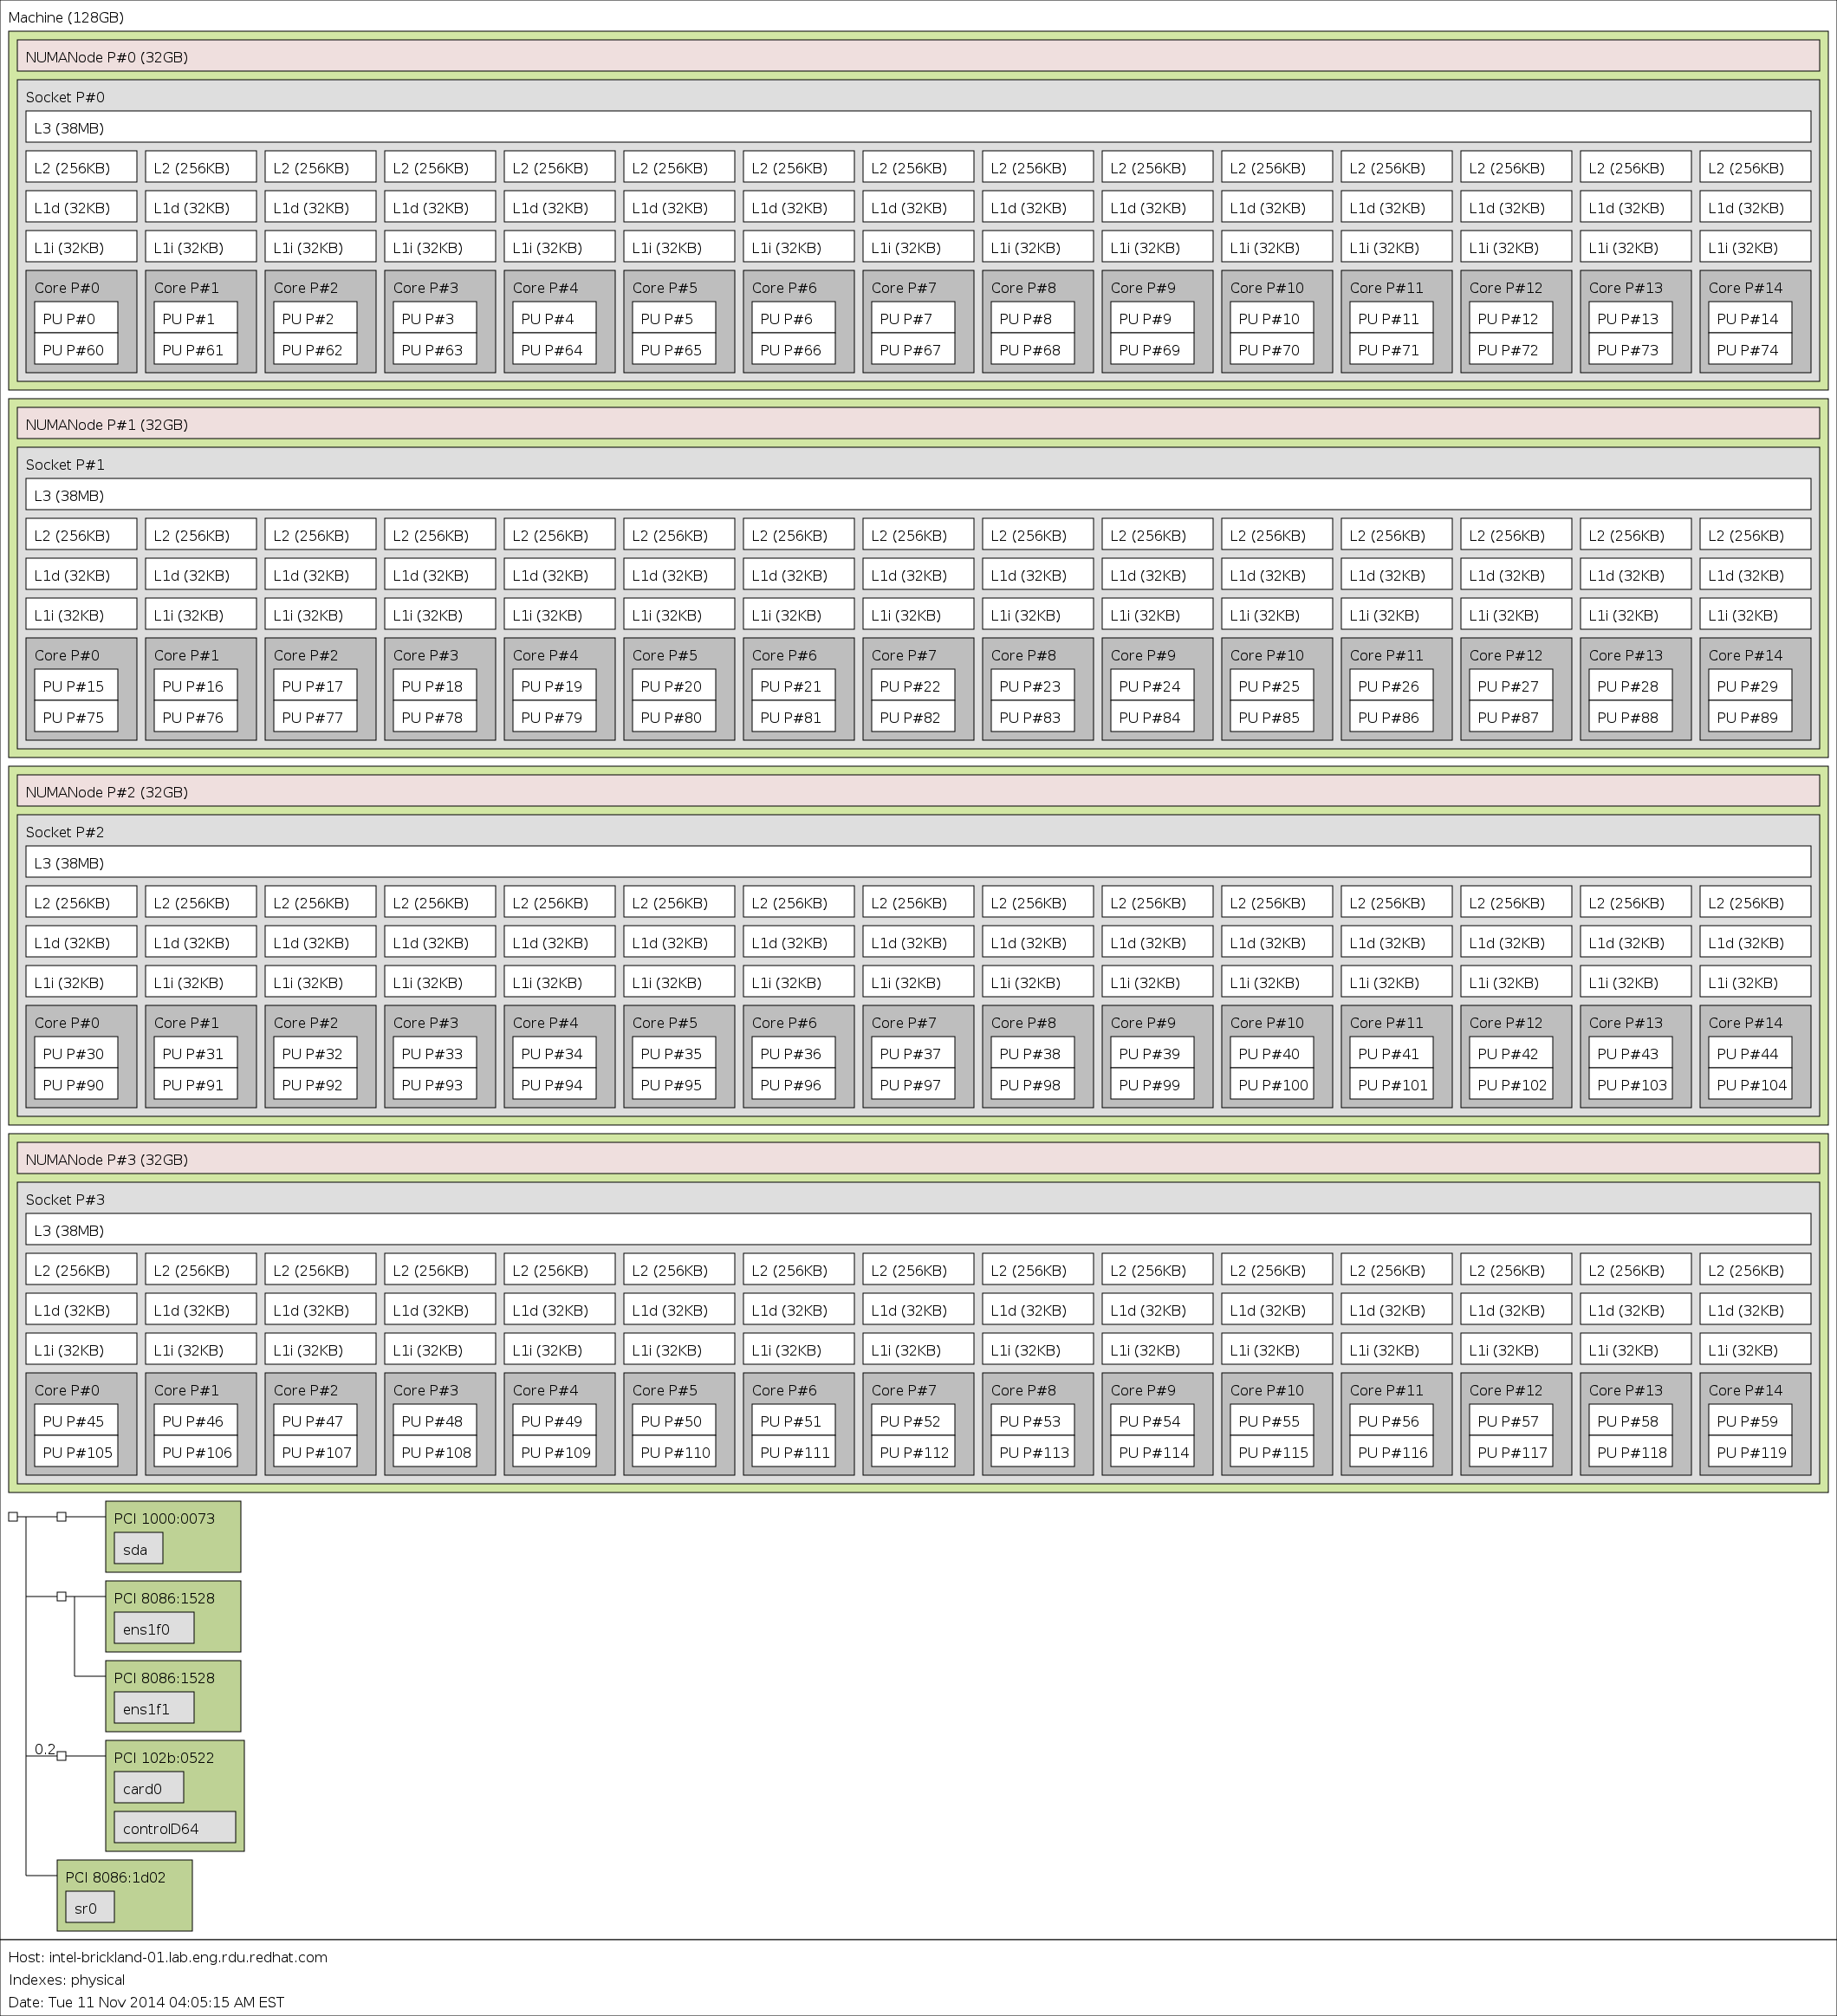
\includegraphics[scale=0.2]{obrazky/lsTOPO-brickland.png}
\caption{Testovaný systém se čtyřmi NUMA uzly a 120 HT jádry}
\label{4 numa NODE system scheme}
\end{figure}


Nejdříve seběhneme linpack benchmark na starší verzi jádra operačního systému a to pro všechny 3 typy běhu (plánovačem řízené, s CPU afinitou, s NUMA afinitou). Pro každý typ běhu běžíme nejdřív 1 instanci linpacku, poté dvě zároveň, čtyři až nakonec 120 (což je celkový počet logických jader v systému viz. obrázek \ref{4 numa NODE system scheme}) instancí najednou. Každý bod, který vynášíme do grafu získáme sečtením dosažených hodnot kflops každé instance.

\newpage

Graf na obrázku \ref{older kernel linpack results} vykresluje hodnoty Kflops dosažené během linpacku na starší verzi jádra. Je zřejmé, že plánovačem dosažené hodnoty (zelená křivka) se výrazně liší od běhů, kde jsme si sami specifikovali afinitu (CPU a NUMA). Nyní seběhneme identický test pro novější jádro operačního systému.

\begin{figure}[ht]
\center
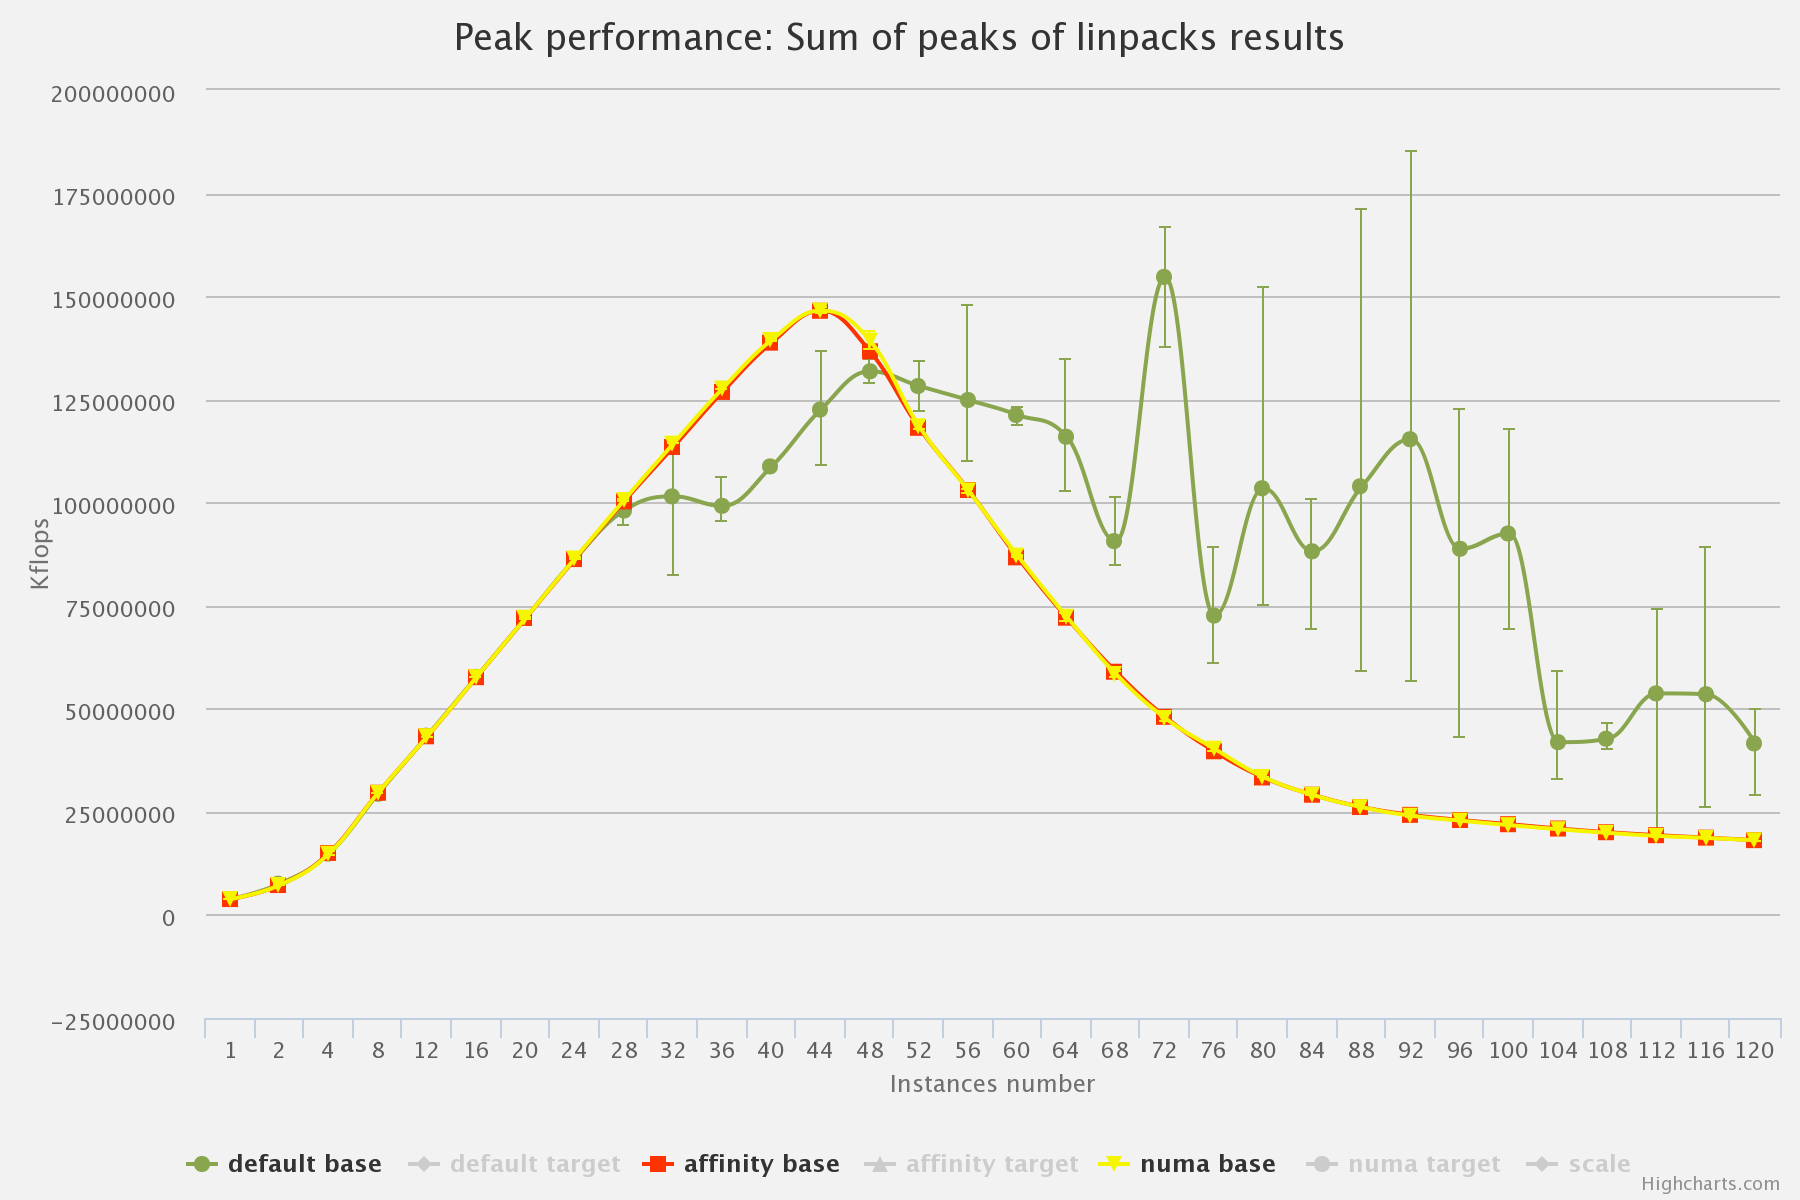
\includegraphics[scale=0.174]{obrazky/LinpackBaseChart.png}
\caption{Výsledky linpacku na starším jádru}
\label{older kernel linpack results}
\end{figure}

Z grafu na obrázku \ref{newer kernel linpack results}, který zobrazuje výsledky běhu linpacku na novějším jádře operačního systému,  zjistíme, že se výsledky pro jednotlivé typy běhu moc neliší. Nyní si vyneseme všech šest křivek do jednoho grafu, abychom viděli, jak rozdílných výsledků dosáhneme u námi testovaných jader. 

\begin{figure}[ht]
\center
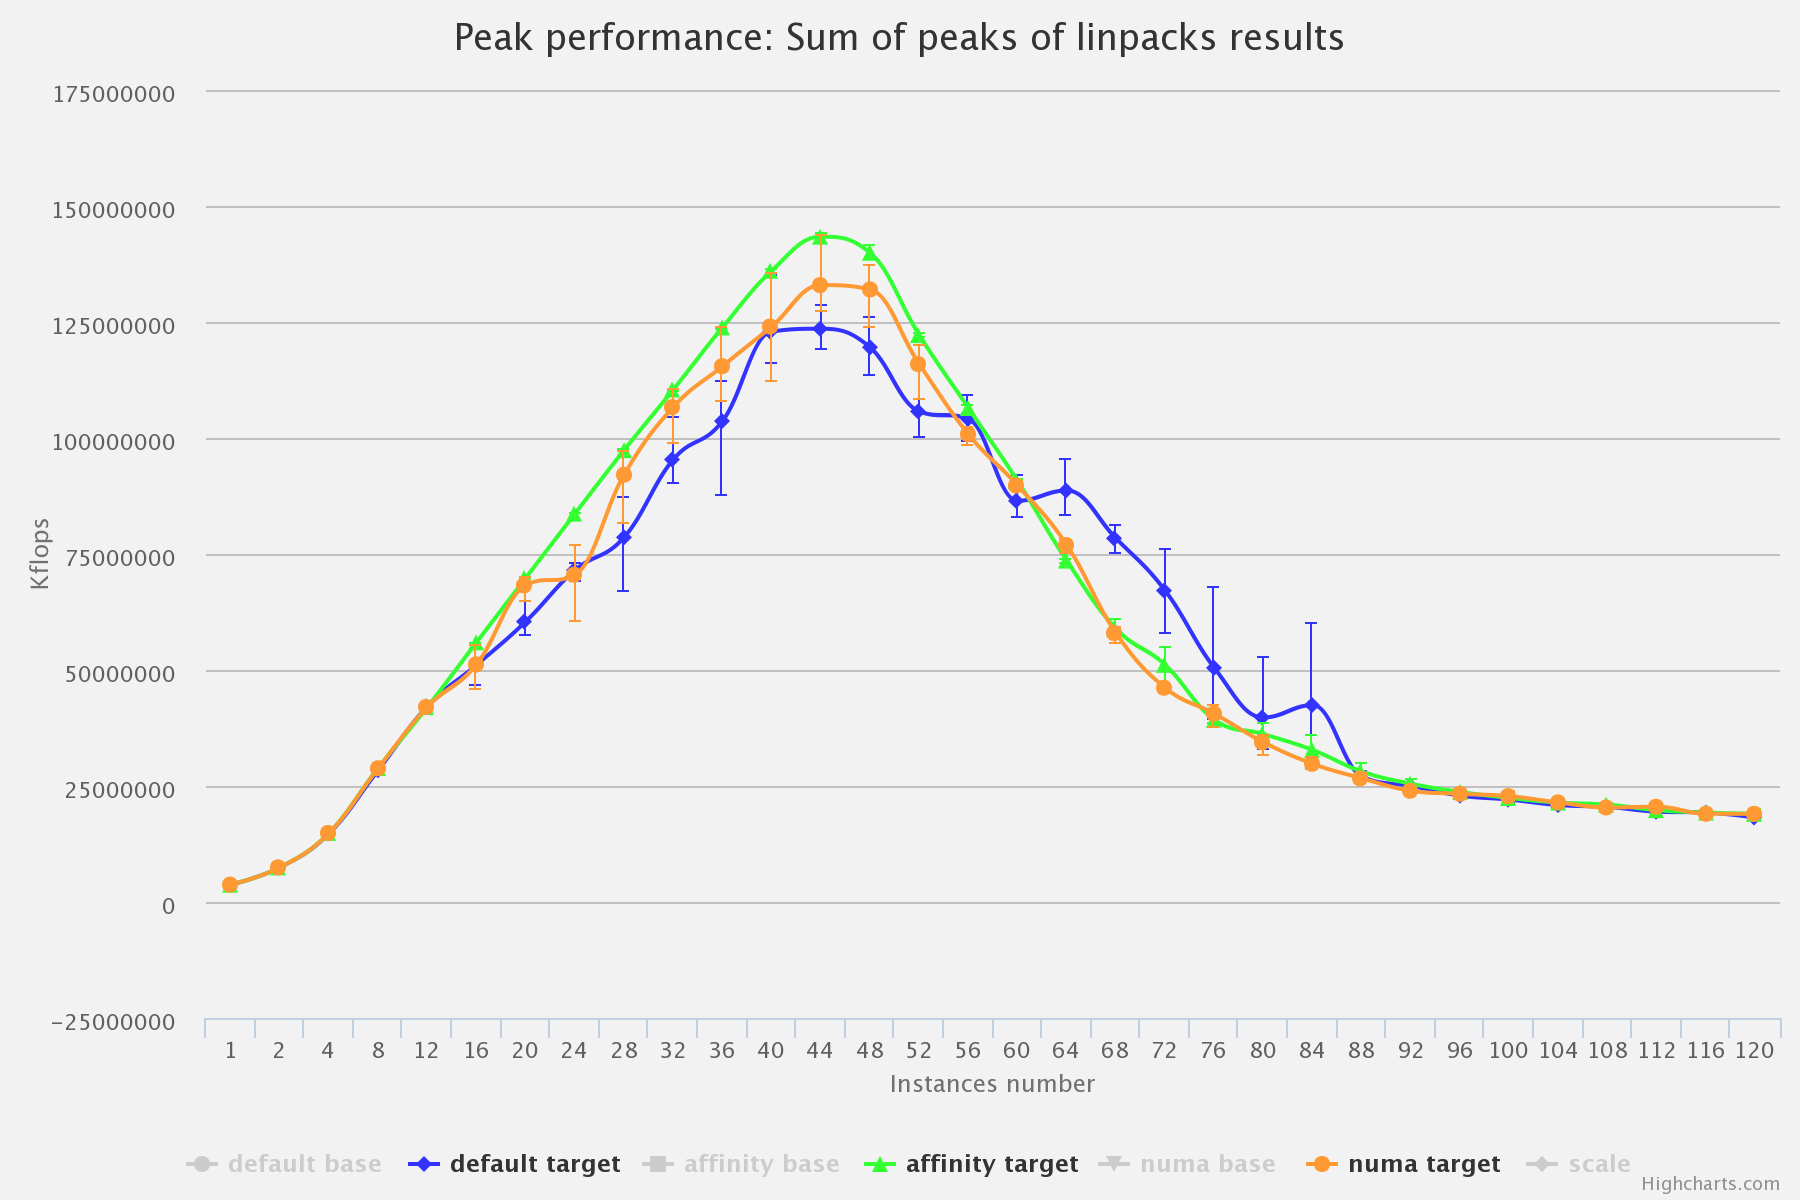
\includegraphics[scale=0.174]{obrazky/LinpackTargetChart.png}
\caption{Výsledky linpacku na novějším jádru}
\label{newer kernel linpack results}
\end{figure}

Zjistíme, že běhy specifikované CPU afinitou se neliší vůbec, běhy specifikované NUMA afinitou se částečně liší a běhy řízené plánovačem se liší dost významně. Zjišťujeme, že kromě toho, že běhy na prvním jádru dosáhly vyšších hodnot kflops, tak mají také veliké rozptyly. Výsledek dosažený na prvním jádru plánovačem se může zdát velice dobrý, ale opak je pravdou. Jelikož jsme volili pro běhy se specifikovanou afinitou právě takové CPU a NUMA uzly, aby byl výsledek co nejlepší, je nemožné, aby plánovač rozmístil úlohy lépe a ty by dosáhly lepšího výsledku. 

\begin{figure}[ht]
\center
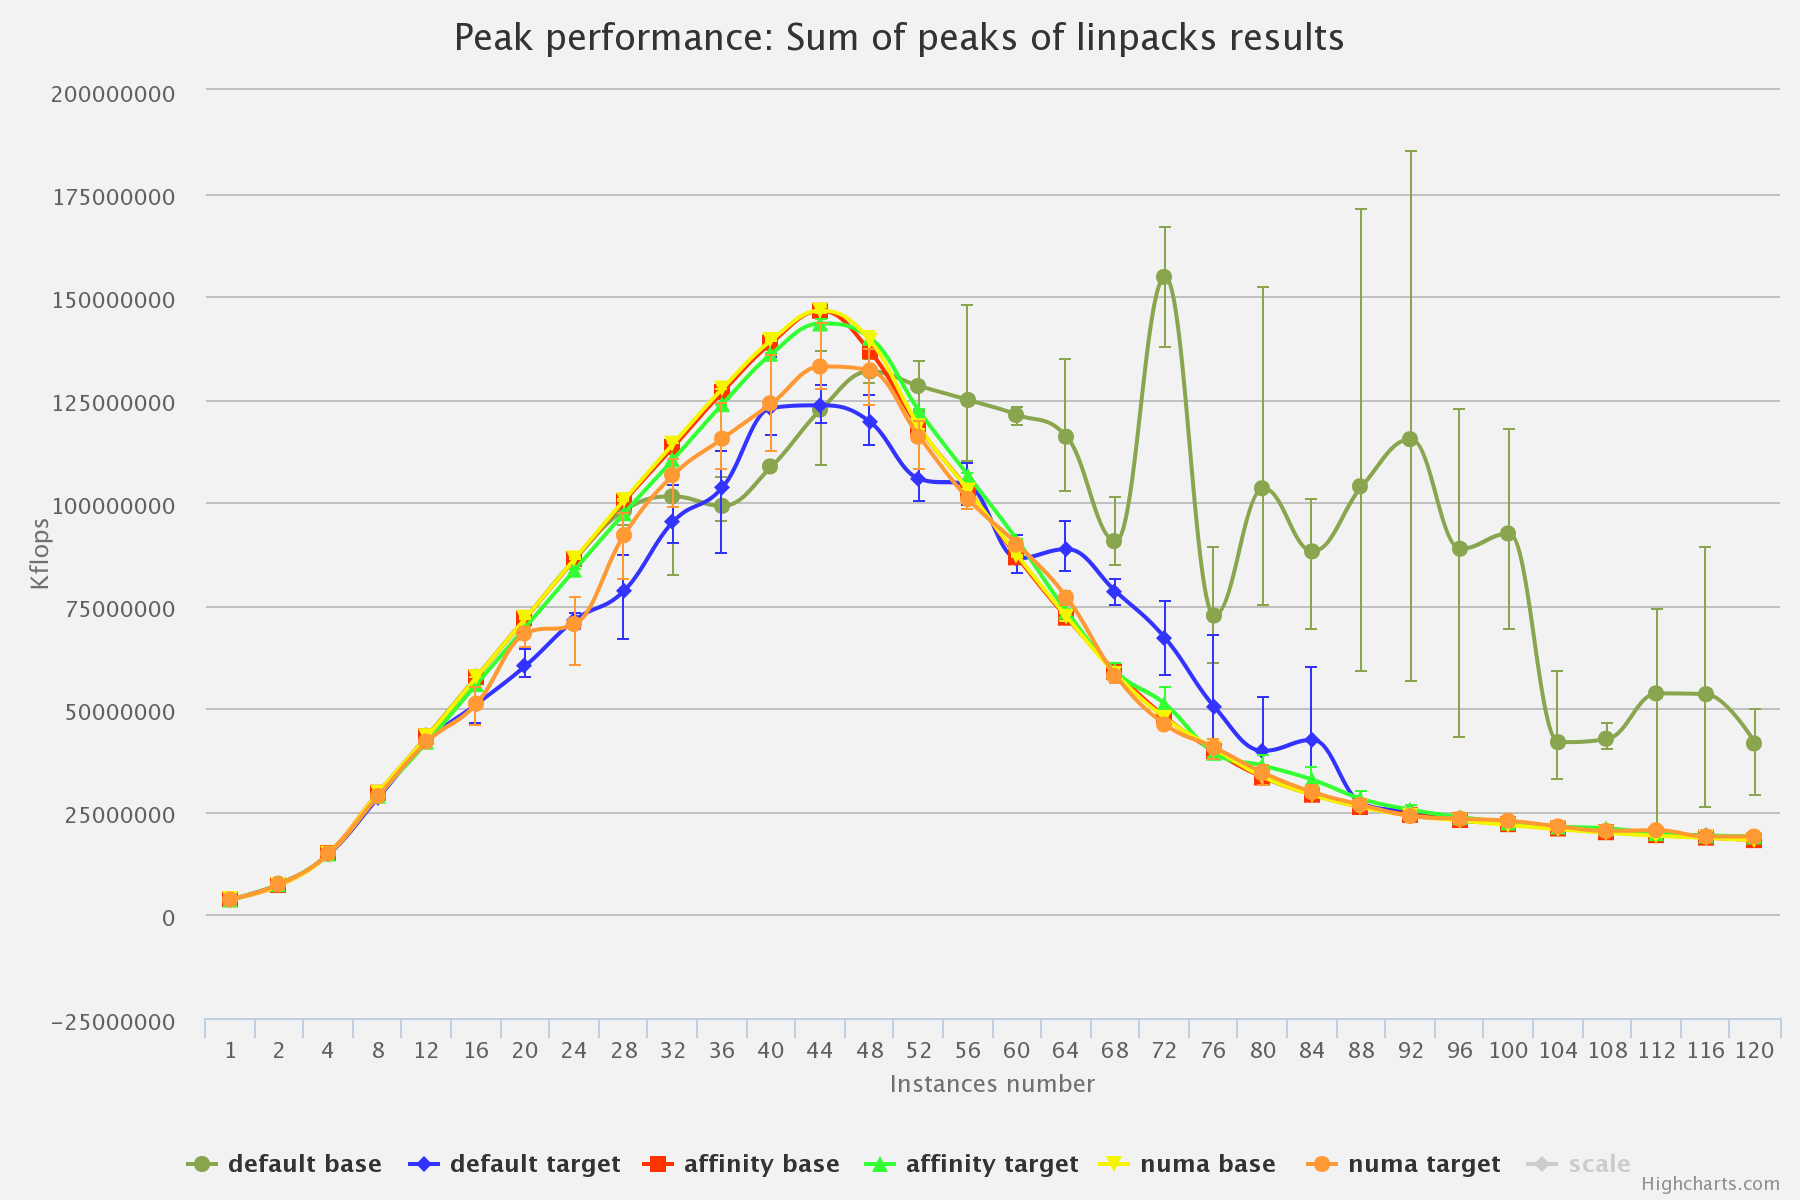
\includegraphics[scale=0.165]{obrazky/LinpackSumChart.png}
\caption{Výsledky ze dvou jader v jednom grafu}
\label{both kernels linpack results}
\end{figure}

Nyní se podíváme na další grafy, které nám odhalí co se při testování stalo. Další graf (z obrázku \ref{timeWaitingOutOfCPU}) znázorňuje kolik času strávily jednotlivé úlohy mimo běh na CPU.

\begin{figure}[ht]
\center
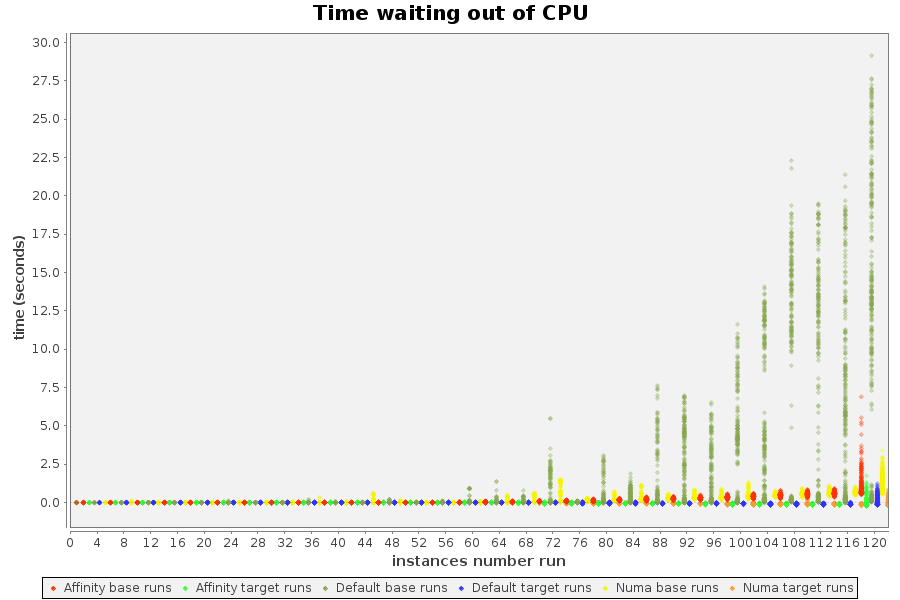
\includegraphics[scale=0.32]{obrazky/timeWaitingOutOfCPU.png}
\caption{Čas strávený mimo CPU}
\label{timeWaitingOutOfCPU}
\end{figure}


\newpage
Další graf (obrázek \ref{total time}) který se nám bude hodit k analýze, je celkový čas běhu jednotlivých úloh (zahrnující i čas strávený mimo CPU).

\begin{figure}[ht]
\center
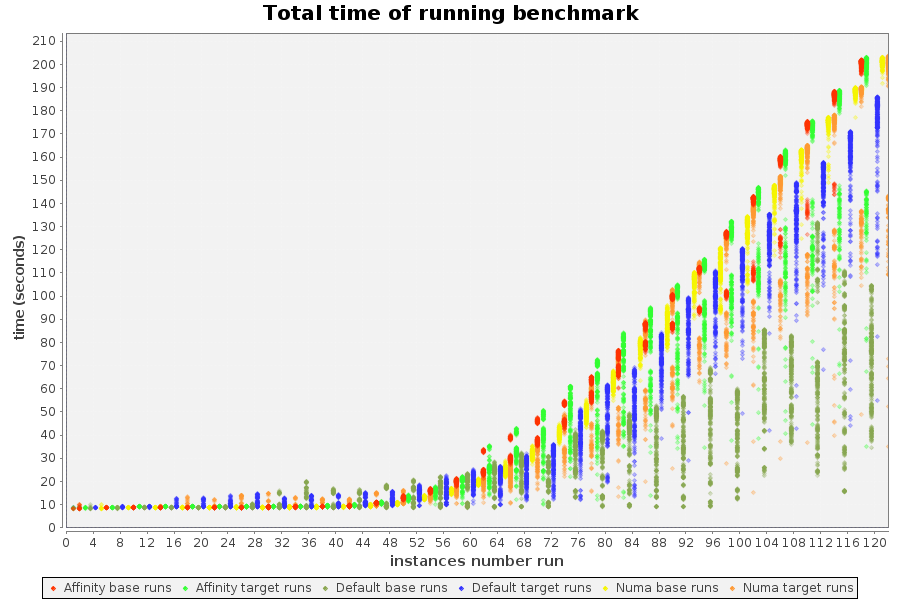
\includegraphics[scale=0.32]{obrazky/totalTime.png}
\caption{Celkový čas běhu úloh}
\label{total time}
\end{figure}

Další zajímavou informací může být zatížení jednotlivých CPU zjišťovaných utilitou mpstat (obrázek \ref{mpstat2}). Zde vidíme značné rozdíly oproti výsledkům dosaženým u druhého testovaného jádra. Výstup je zkrácený ukazuje jen prvních 10 PU. Je zde vidět, že dochází k přesunům úloh na jiná PU, některé úlohy jsou spuštěné později, nebo dokonce je jedna úloha spuštěna, až je druhá dokončena. Toto samozřejmě úloze nechá celou vyrovnávací paměť a úloha pak seběhne rychleji. Toto řešení nemá nicméně nic společného s férovostí. 

\begin{figure}[ht]
\caption{mpstat zkrácený sumarizovaný výpis}
\center
\label{mpstat2}

\begin{Verbatim}[frame=single]

        0  1  0  1  0  0  0 49 ** 85  0 19 ** ** ** 85 
        1  0  0  0  0  0  0 37 ** ** ** 79 ** ** ** 79
        2  0  0  0  0  0  0 50 ** ** ** 86 76 ** ** ** 
        3  0  0  0  0  0  0  0  0  0  0  0  0  0  0  0 
        4  1 ** ** ** ** ** 52  0  0  0  0  0  0  0  0
        5  1 ** ** ** ** ** 54  0  0  0  0  0  0  0  0
        6  1  1  1  0  0  1  0  0  3 ** ** ** ** 89 **
        7  1 ** ** ** ** ** ** ** 97 ** ** ** 95 78 **
        8  1  1  0  0  0  0  1  0  0 96 ** ** ** 81 **
        9  1 ** ** ** ** ** ** ** 99 82 ** ** ** 18  0
       10  1 ** ** ** ** ** ** ** 82  0  0  0  0  0  0
      
\end{Verbatim}
\end{figure}
\newpage

\noindent
\subsubsubsection{Příklad na umístění nově vzniklého procesu a jeho dat na stejný NUMA uzel}
\label{PerfBenchResultExample}

\noindent
Dále nás zajímá kde plánovač umisťuje paměť procesu a kde samotný proces. K tomu účelu použijeme perf bench benchmark. Tento příklad ukazuje nevhodné kopírování paměti mezi NUMA uzly. Napravo na obrázku \ref{PerfBenchResult} je paměť úloh, nalevo je zobrazeny rozmístění úloh na NUMA uzlech. V tomto příkladu jsou spuštěny 2 vlákna celkem mají 8GB paměti a běží 20 min. Až po 6ti minutách dochází k rozdělení dat a procesů na 2 NUMA uzly. 

\begin{figure}[ht]
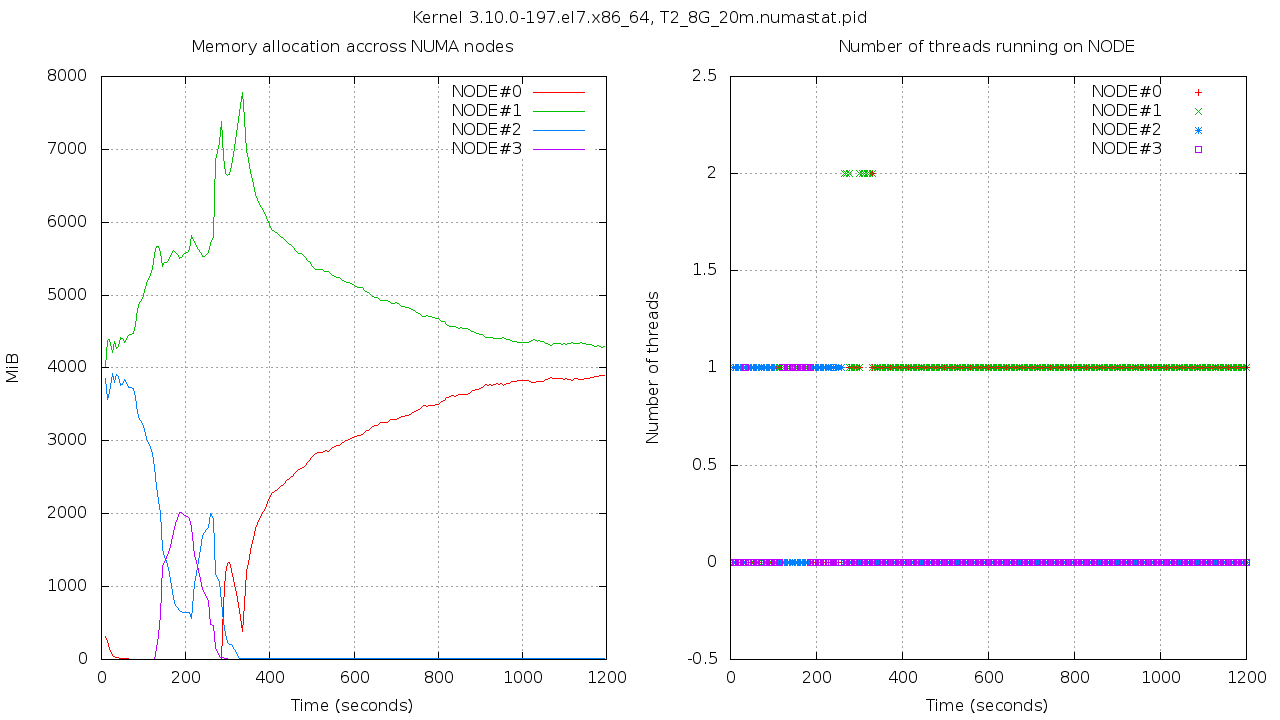
\includegraphics[scale=0.30]{obrazky/PerfBenchResult.png}
\caption{Graf znázorňující současný běh dvou úloh}
\label{PerfBenchResult}
\end{figure}

\section{Závěr}
Po bližším obeznámení se s plánovačem úloh jsem došel k přesvědčení, že návrh plánovače byl precizně navrhnut a implementován po NUMA vyvažování. Připadá mi, že NUMA vyvažování nebylo přidáno do kódu v duchu návrhu celého plánovače, hlavně tedy třídy pro plánování obyčejných úloh. Kód NUMA vyvažování je dlouhý, postrádám v něm jakýsi koncept, vadí mi heuristika. Překvapilo mě, že se při NUMA vyvažování kalkuluje s pomocí konstant jako například výpočetní síla skupiny procesorů, nebo jak získává historii přístupu na stránky. Tu určí tak, že dosavadní přístupy vydělí dvěma. Jsem přesvědčen, že tvůrci NUMA vyvažování udělali chybu v tom, že se NUMA vyvažování realizuje dvěmi různými funkcemi, které si nejsou vůbec podobné a spouštějí při dvou událostech (jedna periodicky, druhá při přístupu na uzamčené stránky paměti). To očividně vede k neustálému migrování úloh a jejich dat z jednoho NUMA uzlu na druhý. Od vývojáře NUMA plánovače jsem byl informován, že toto je slabina současného plánovače a že se nyní vymýšlí, jak tuto slabinu odstranit. 

\nocite{*}

%\printglossary
%\printbibliography


\printindex


\begin{thebibliography}{9}
  \bibitem{vseeker}{\em Volker Seeker:}
               {Process scheduling in Linux} \\ 
               University of Edinburgh 2013
%	\hyperref[name]{}
%	\href{http://criticalblue.com/news/wp-content/uploads/2013/12/linux\_scheduler\_notes\_final.pdf}{URL link to Process scheduling in Linux document}
  \bibitem{kernelorg}{\em Dokumentace na www.kernel.org 
               k linuxovému plánovači}\\
               \texttt{https://www.kernel.org/doc/Documentation/scheduler/}
  \bibitem{ibm}{\em IBM developerworks článek} \\
		\texttt{http://www.ibm.com/developerworks/library/} \\
		\texttt{l-completely-fair-scheduler/}
  \bibitem{linuxjournal}{\em Článek z linuxjournal} \\
		\texttt{http://www.linuxjournal.com/magazine/completely-fair-scheduler}
  \bibitem{kernel mailing lists}{\em Emaily věnované plánování z lwn.net a lkml.org} \\ 
		\texttt{https://lkml.org} \\
		\texttt{https://lwn.net}
  \bibitem{RRIEL}{\em Prezentace od Rika van Riela} \\
		Interní RedHat prezentace od jednoho z vývojářů vyvažovacího algoritmu v CFS plánovači

\end{thebibliography}


\end{document}



